%%%%%%%%%%%%%%%%%%%%%%%%%%%%%%%%%%%%%%%%%%%%%%%%%%%%%%%%%%%%%  
%
% SZABLON PRACY DYPLOMOWEJ
% WYMAGANIA ISE EITI PW
% AUTOR: Królik
% OPARTE NA SZABLONACH AUTORSTWA: Paszciora, Mastera & Kuchara
% 2011
% 
%%%%%%%%%%%%%%%%%%%%%%%%%%%%%%%%%%%%%%%%%%%%%%%%%%%%%%%%%%%%%
\author{Michał Haponiuk}
\title{Przeglądarka genomu}
\date{\today}

\documentclass[a4paper,12pt,oneside]{mwrep}  %bylo report
\usepackage[utf8]{inputenc} %ISO-8859-2 
\usepackage[polish]{babel} 
\usepackage{times} 
\usepackage[T1]{fontenc} 
\usepackage[MeX]{polski} 
\usepackage[pdftex]{color,graphicx} 
\usepackage{pdfpages} 
\usepackage{fancyhdr} %numery stron po zewnętrznej 
\usepackage{wrapfig}
\usepackage{caption}
\usepackage[bookmarks,unicode
			% odkomentowanie linijki poniżej usuwa kolorowe ramki w linkach
			%,colorlinks,citecolor=black,filecolor=black,linkcolor=black,urlcolor=black
			]{hyperref} 
\usepackage{titlesec} 
%\usepackage[dvi-ps]{graphicx}

%marginesy 
\usepackage[ bindingoffset = 1cm, hmargin = 2cm, vmargin = 2cm]{geometry} 
%interlinia 
\linespread{1.5} 

\widowpenalty=10000 % ostatni wierszrkapitu nie zostanie przeniesiony na następną stronę 
\clubpenalty=10000 % pierwszy wiersz akapitu nie będzie kończył strony (nie używam tego ustawienia)
\hbadness= 1450 %% zmniejsza liczę wyświetlanych ostrzeżeń (można zwiększyć, ale bez przesady)
\hfuzz = 0pt %% tekst może sterczeć ma marginesie na 1,5pt (ok. 0,5mm)

\clubpenalty=10000 %nie pozostawia sierot
\brokenpenalty=10000 %nie dzieli stron je»eli podziaª wyrazu
\sloppy %zakaz wydªu»ania lini

%wcięcia 
\setlength{\parindent}{1cm} 
\setcounter{secnumdepth}{2} %only sections and subsections are numbered 
\setcounter{tocdepth}{2} %table of contents shows up to three levels 



%eiti 
%rozdział 16pt, pogrubiona, kapitalki, interlinia 2 

\titleformat{\chapter}[hang] 
{\Large\bfseries}{\thechapter}{10pt}{\Large\bfseries} 
\titlespacing{\chapter}{0pt}{1em}{1em} 

%podrozdział 12pt, pogrubiona, kapitalki, il 2 
\titleformat{\section}[hang] 
{\normalfont\bf}{\thesection}{10pt}{\normalfont\large\bf} 
\titlespacing{\section}{0pt}{1em}{1em} 

%punkt 12pt, pogrubiona, il 2 
\titleformat{\subsection}[hang] 
{\normalfont\bf}{\thesubsection}{10pt}{\normalfont\large\bf} 
\titlespacing{\subsection}{0pt}{1em}{1em} 


%podpunkt 12pt, il 2 
\titleformat{\subsubsection}[hang] 
{\normalfont}{\thesubsubsection}{10pt}{\normalfont\bf} 
\titlespacing{\subsubsection}{0pt}{1em}{1em} 

\titleformat{\paragraph}[hang] 
{\normalfont}{\theparagraph}{10pt}{\normalfont\it} 
\titlespacing{\paragraph}{15pt}{1em}{1em} 

\renewcommand{\contentsname}{Spis treści} 
\renewcommand{\refname}{Bibliografia}


\begin{document} 

%%%%%%%%%%%%%%%%%%%%%%%%%%%%%%%%%%%%%%%
%STRONA TYTUŁOWA
%%%%%%%%%%%%%%%%%%%%%%%%%%%%%%%%%%%%%%%
\begin{titlepage} 

% Logo Politechniki Warszawskiej
\begin{figure*}
        
\includegraphics[width=2.5cm]{grafika/logo_pw} \hfill
        
\includegraphics[width=2.5cm]{grafika/logo_weiti}
\end{figure*}

\begin{center}

\LARGE{\textbf{POLITECHNIKA WARSZAWSKA}}\\
\Large{Wydział Elektroniki i~Technik Informacyjnych}\\
\large{Instytut Informatyki}				%%% Instytut

\vfill

\vfill
\huge \textbf{Michał Haponiuk}\\  						 %%%Imie i nazwisko
\large{nr albumu: 249371}\\[1cm] 						 %%% numer albumu

\textsc{\Large Praca Dyplomowa Inżynierska}\\[1,5cm]     %%% rodzaj pracy

\huge \textbf{Przeglądarka genomu}\\[2cm] %%% Tytuł pracy

\vfill

\begin{flushright}
\large{Praca wykonana pod kierunkiem\\
dr~hab.~inż.~Robert~Nowak}\\[1cm] 
\end{flushright}


% Bottom of the page
\large{Warszawa, \today}

\end{center}
\end{titlepage} 

\pagestyle{empty}
\cleardoublepage 


\def\abstract{
   \vfil
   \begin{center}%
	   {\bfseries {\Large \abstractname}}%
   \end{center}
   \quotation
   }
   
   \def\endabstract{\par
   \endquotation
   }
   \thispagestyle{empty}
   
%%%%%%%%%%%%%%%%%%%%%%%%%%%%%%%%%%%%%%%%%%%%%%%%%%%%%%%%%%%%%%  
% ZYCIORYS
%%%%%%%%%%%%%%%%%%%%%%%%%%%%%%%%%%%%%%%%%%%%%%%%%%%%%%%%%%%%%
{
\begin{wrapfigure}[5]{l}{6cm}
\begin{center}
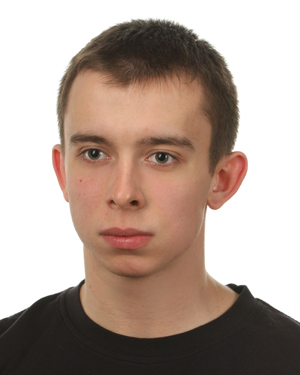
\includegraphics[width=4cm]{grafika/HAPONIUK_MICHAL.jpg}
\end{center}
\end{wrapfigure}


\setlength{\parindent}{0pt} %likwiduje wciecie w akapicie
\setlength{\baselineskip}{1.6\baselineskip}
Imię i nazwisko: \hfill Michał Haponiuk\\
Kierunek: \hfill Informatyka\\
Specjalność: \hfill Inżynieria Systemów Informatycznych\\
Data urodzenia: \hfill 3 kwietnia 1992\\
Data rozpoczęcia studiów: \hfill 20 luty 2012\\


%\vspace{1cm}
\begin{center}
{\bfseries {\Large Życiorys}}%
%\Large ŻYCIORYS
\end{center}
\vspace{0.5cm}
\setlength{\baselineskip}{0.625\baselineskip}
Urodziłem się 3 kwietnia 1992 roku w~Kielcach. W~2008 roku rozpocząłem naukę w~II Liceum Ogólnokształcącym im. Jana Śniadeckiego w~Kielcach, w~klasie o~podstawie programowej w~zakresie rozszerzonym z~matematyki, informatyki, fizyki i~astronomii . W~2011 roku uzyskałem wykształcenie średnie oraz świadectwo dojrzałości. W~następnym roku zostałem przyjęty na studia stacjonarne pierwszego stopnia, na Wydziale Elektroniki i~Technik Informacyjnych, kierunku Informatyka. Po dwóch latach studiów, obrałem specjalność Inżynierii Systemów Informatycznych.

\vspace{0.5cm}
\begin{flushright}
\parbox[pos]{6cm}{
\setlength{\baselineskip}{0.625\baselineskip}
\dotfill \\
\centering Podpis studenta
}
\end{flushright}


\vspace{1cm}
%\vspace
\setlength{\baselineskip}{1.4\baselineskip}
EGZAMIN DYPLOMOWY\\
Złożył egzamin dyplomowy w~dniu \dotfill 2016 r.\\
z wynikiem \dotfill \\
Ogólny wynik studiów: \dotfill \\
Dodatkowe wnioski i~uwagi Komisji: \dotfill \\
\makebox[1\columnwidth]{\dotfill}
\makebox[1\columnwidth]{\dotfill}

}
\newpage	

\cleardoublepage 

%%%%%%%%%%%%%%%%%%%%%%%%%%%%%%%%%%%%%%%%%%%%%%%%%%%%%%%%%%%%%   
% STRESZCZENIA
%%%%%%%%%%%%%%%%%%%%%%%%%%%%%%%%%%%%%%%%%%%%%%%%%%%%%%%%%%%%%
\begin{abstract}

	\begin{center}
	{\bfseries Przeglądarka genomu}\\[0.3cm]
	\end{center}
	
\setlength{\parindent}{0pt}
Celem niniejszej pracy inżynierskiej było utworzenie aplikacji pozwalającej na przechowywanie i~interaktywne przeglądanie danych genetycznych pozyskiwanych z~sekwencjonowania genomów. Praca rozpoczyna się wprowadzeniem czytelnika w~świat bioinformatyki i~zagadnień związanych z~przeglądarkami genomów. Następnie został opisany proces projektowania i~implementacji, oraz omówione zostały użyte technologie i~narzędzia, ułatwiające realizację programu. Oprogramowanie było tworzone z~myślą o~możliwości dalszego rozszerzania i~rozwoju.
\vfill
Słowa kluczowe: przeglądarka genomów, bioweb, bioinformatyka, sekwencje
\bigbreak
\noindent\rule{\linewidth}{0.5pt} \\ 
\end{abstract}

\renewcommand\abstractname{Abstract}
\begin{abstract}
	\begin{center}
	{\bfseries Genome viewer}\\[0.3cm]
	\end{center}

\setlength{\parindent}{0pt}
The purpose of this thesis was to create an application for storing and interactive browsing genetic data obtained from genome sequencing. The work begins with an introduction the reader into the world of bioinformatics and issues related to genome browsers. Thereafter, it was described the process of design and implementation. It discusses the technologies and tools which simplify accomplishment of the program. The software was written specifically about the possibility of further development.
\vfill
Keywords: genome viewer, bioweb, bioinformatics, sequences
\end{abstract}

\newpage	
\thispagestyle{empty}
\cleardoublepage 

%%%%%%%%%%%%%%%%%%%%%%%%%%%%%%%%%%%%%%%%%%%%%%%%%%%%%%%%%%%%%  
% SPIS TRESCI
%%%%%%%%%%%%%%%%%%%%%%%%%%%%%%%%%%%%%%%%%%%%%%%%%%%%%%%%%%%%%
\tableofcontents

\newpage



%\cleardoublepage
\pagestyle{plain}

%%%%%%%%%%%%%%%%%%%%%%%%%%%%%%%%%%%%%%%%%%%%%%%%%%%%%%%%%%%%%  
% PRACA WLASCIWA
%%%%%%%%%%%%%%%%%%%%%%%%%%%%%%%%%%%%%%%%%%%%%%%%%%%%%%%%%%%%%
\chapter{Cel i~zakres pracy}
Informatyka jest aktualnie bardzo rozległą dziedziną nauki, z~osiągnięć której szeroko korzystają inne dyscypliny naukowe a~wśród nich genomika - nauka zajmująca się analizą genomu, której celem jest poznanie sekwencji materiału genetycznego, mapowanie genomu oraz określenie wszelkich zależności i~interakcji wewnątrz genomu.

Cechy każdego żywego organizmu zapisane są na nośniku informacji genetycznej, którym w~komórkach posiadających jądro komórkowe jest kwas dezoksyrybonukleinowy (DNA). DNA składa się z~nukleotydów, których kolejność występowania warunkuje cechy organizmu. Kompletny zapis informacji genetycznej nosi nazwę genomu.

Dokładną budowę chemiczną z~przestrzennym modelem cząsteczki DNA udało się opracować stosunkowo niedawno, bo w~1953 r. a~odkrywcy - James D. Watson i~Francis Circk, otrzymali Nagrodę Nobla. Jako pierwszy ukończono projekt poznania genomu bakteriofaga \begin{math}
\Phi
\end{math}-X174, mającego 5368 par zasad. Zsekwencjonował go Frederick Sanger w~1977 r. Pierwszy ukończony projekt dotyczący bakterii to projekt poznania genomu \emph{Haemophilus influenzae} wykonany w~TIGR (\emph{The Institute for Genomic Research}) w~1995r. W~1988 roku grupa naukowców z~18 państw rozpoczęła badania nad ludzkim genomem w~ramach projektu HGP (\emph{Human Genom Project}). Wstępny opis genomu człowieka opublikowano w~2000 roku. Badacze odkrywają genomy także i~innych organizmów (bakterii, roślin i~zwierząt) a~liczba ukończonych projektów ciągle wzrasta. 
Dostępność całych, często obszernych genomów organizmów, stworzyła potrzebę wizualizacji, zaspokajaną przez zastosowanie przeglądarek.
Zaproponowana przeze mnie przeglądarka genomu wpisuje się w~katalog istniejących projektów umożliwiając wysłanie i~przeglądanie danych zlokalizowanych na komputerze użytkownika. %\cite{nature ,wikipedia-pl} %wikipedia genom

\section{Układ pracy}
Tekst składa się z~pięciu rozdziałów. Na początku pracy zapoznaję czytelnika z~podstawowymi zagadnieniami dotyczącymi bioinformatyki. W~trakcie wprowadzenia w~problematykę genomiki, opisuję pojęcia biologiczne bezpośrednio związane z~projektowaną przeglądarką. Przedstawiam rys historyczny pokazujący jak rozwijał się przemysł bioinformatyczny w~XX wieku. Poruszam kwestie technologii używanych w~ teraźniejszych przeglądarkach genomów oraz przedstawiam rozwiązania dostępne na rynku. W~kolejnym rozdziale opisuję wymagania funkcjonalne i~niefunkcjonalne stawiane projektowanemu systemowi oraz opowiadam o~zaprojektowanej architekturze i~użytych technologiach. Omawiam również wybrane kluczowe decyzje implementacyjne. Czwarty rozdział zawiera demonstrację funkcjonalności aplikacji. Pracę kończy podsumowanie wraz z~opisem potencjalnych możliwości rozwoju programu.

\chapter{Przeglądarki genomów}

Bioinformatyka jako dziedzina nauki łączy w~sobie informatykę i~matematykę w~celu przetwarzania danych biologicznych. Dynamiczny rozwój biologii molekularnej oraz~genomiki przyczynił się do powstania olbrzymiej ilości informacji. Konsekwencją jest utworzenie i~zarządzanie rozwiniętymi bazami danych, w~których mogą być gromadzone i~sprawnie przeglądane dane biologiczne. Wykorzystywanie narzędzi bioinformatycznych istotnie redukuje czas projektowania i~przeprowadzania doświadczeń oraz zmniejsza koszty. Na biologach została wywarta presja, aby w~swojej pracy korzystali z~komputerów i~informatyki na etapach gromadzenia, wydobywania oraz~przetwarzania informacji zawartych w~DNA (rys.\ref{model-dna}), RNA i~białkach. Cząsteczki te mogą być opisywane przez sekwencje symboli. %\cite{pl-wiki-bioinf}

\begin{figure}[!h]
\centering

\includegraphics[width=0.83\textwidth]{grafika/DNA2}
%zdjecie z~http://wideshut.co.uk/wp-content/uploads/2013/07/DNA.jpg
%zdjecie https://forensicdnaconsulting.files.wordpress.com/2013/07/canstockphoto2267476.jpg
\caption{Prosty model DNA.}
\vspace{-0.8cm}
\caption*{\scriptsize Źródło: \url{https://forensicdnaconsulting.files.wordpress.com/2013/07/canstockphoto2267476.jpg}}
\label{model-dna}
\end{figure}

Przeglądarki genomów są narzędziem, które upraszczają i~porządkują dane związane z~genomem danego organizmu. Obecnie przeglądarki posiadają graficzny interfejs użytkownika. Umożliwiają naukowcom wizualizacje całych genomów z~dodatkowymi informacjami pozyskiwanymi zwykle z~wielu źródeł\footnote{Dane porównawcze (drzewa filogenetyczne, zmienności), laboratoryjne badania analityczne (sekwencje, skany), odnośniki do innych baz, przetworzone dane laboratoryjne.}. Różnią się one od zwykłych biologicznych baz danych, gdyż dane są opisane współrzędnymi w~genomie. Rysunek \ref{przykladowa-przegladarka-genomu} ilustruje typową wizualizację genomu dla przeglądarki UCSC (roz.\ref{UCSC}). Można przyjąć, że obrazuje się sekwencje wraz z~adnotacjami.

\begin{figure}[h]
\centering
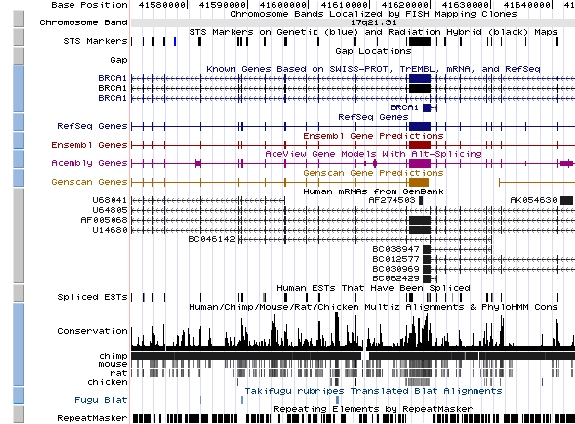
\includegraphics[width=0.75\textwidth]{grafika/browsershot_ucsc}
%zdjecie z https://genomics.soe.ucsc.edu/research/browser_overview
\caption{Fragment typowej wizualizacji genomu przeglądarki UCSC. Wyświetlany zakres danych jest ułożony pionowo. Na samej górze, pokazany jest numer i~pozycja na chromosomie. Kilka poniższych wierszy ilustruje dane dotyczące genów, które zostały doświadczalnie znalezione lub przewidziane różnymi metodami. Kolejne wiersze dotyczą poziomu ekspresji genów, a~pod nimi znajduje się porównanie z~genomami innych gatunków.}
\vspace{-0.8cm}
\caption*{\scriptsize Źródło: \url{https://genomics.soe.ucsc.edu/research/browser_overview}}
\label{przykladowa-przegladarka-genomu}
\end{figure}

\section{Mapowanie genomów}
Przeglądarka genomów opisuje położenie elementów w~genomie, poczynając od chromosomów. Następnie ustalane jest położenie sekwencji lub adnotacji wewnątrz chromosomu co tworzy mapę. Uwzględniając zjawisko rekombinacji rozróżniamy \emph{mapy genetyczne}, wyrażające oddalenie między specyficznymi sekwencjami (markerami), oraz \emph{mapy fizyczne}, określające pozycję genów w~sposób bezpośredni, jako indeks. Rekordy zawarte w~obu typach map uzupełniają się nawzajem, będąc podstawą do kolejnych badań nad ukształtowaniem i~strukturą chromosomów. %\cite{e-biotech-map-gen}

\subsection{Mapy genetyczne}
Mapy genetyczne, wykorzystując analizę sprzężeń genetycznych, umożliwiają określenie rozłożenia genów i~innych rozpoznawalnych markerów (sekwencji) w~genomie oraz ustalają odległość genetyczną między nimi. Miara wyrażana jest w~centymorganach\footnote{Jeden cM  to taka odległość pomiędzy dwoma loci, że szansa na ich rozdzielenie w~procesie rekombinacji genetycznej w~ciągu jednego pokolenia (podczas jednorazowego wydarzenia, np. crossing-over) wynosi 1\%.Centymorgany nie odzwierciedlają bezwzględnej odległości pomiędzy obszarami chromosomu zajmowanymi przez gen, ponieważ częstość rekombinacji jest różna w~różnych rejonach chromosomów, na różnych chromosomach oraz w~różnych organizmach.%\cite{pl-wiki-cM}
}
(cM). %\cite{e-biotech-map-gen}

\subsection{Mapy fizyczne}
Techniki biologii molekularnej są wykorzystywane w~mapach fizycznych w~celu bezpośredniego usytuowania poszczególnych sekwencji DNA w~genomie. Jednostką w~tych mapach są pary zasad\footnote{Para zasad to dwie komplementarne zasady nukleotydów dwóch różnych nici kwasu nukleinowego, połączone wiązaniem wodorowym, zgodnie z~następującą regułą: adenina(A) tworzy zawszę podwójne wiązanie wodorowe z~tyminą (T) a~cytozyna(C) tworzy potrójne wiązanie wodorowe z~guaniną (G). %\cite{e-biotech-encykl-pz}
} (pz). Tablica~\ref{lancuchy_DNA} przedstawia mapę dwóch komplementarnych łańcuchów DNA. Oba mają długość 15 pz. %\cite{e-biotech-map-gen}

\begin{table}[!hb]
	\begin{center}
		\begin{tabular}{c|c|c|c|c|c|c|c|c|c|c|c|c|c|c|c|c|c|c|}\cline{2-16}\emph{Łańcuch 1}&
		\verb|A|&\verb|T|&\verb|C|&\verb|G|&\verb|A|&\verb|T|&\verb|T|&\verb|G|&\verb|A|&\verb|G|&\verb|C|&\verb|T|&\verb|C|&\verb|T|&\verb|A|\\ \cline{2-16}
		\emph{Łańcuch 2} &\verb|T|&\verb|A|&\verb|G|&\verb|C|&\verb|T|&\verb|A|&\verb|A|&\verb|C|&\verb|T|&\verb|C|&\verb|G|&\verb|A|&\verb|G|&\verb|A|&\verb|T|\\ \cline{2-16}
		\end{tabular}
	\end{center}
\caption{Mapa dwóch komplementarnych łańcuchów DNA.}
\label{lancuchy_DNA}
\end{table}

\subsection{Pojęcia}
W pracy używam wybranych pojęć biologicznych:
\begin{itemize}
\item \textbf{Chromosom} jest strukturą zawierającą materiał genetyczny komórki. Zbudowany jest głównie z~pojedynczej olbrzymiej liniowej cząsteczki DNA. Podczas podziału jądra chromosomy przyjmują zwartą strukturę i~stają się widoczne w~mikroskopie jako pojedyncze obiekty. Struktura chromosomu nie jest niezmienna, podlega on bowiem zmianom zwanym mutacjami\footnote{Mutacje genomowe powodują zaburzenia genetyczne lub zespoły chorobowe, takie jak zespół Downa czy zespół Turnera.}. \cite{wikipedia-pl, pwn-encyklopedia} %wiki-pl: chromosom, encyklopedia pwn: chromosomy
%co to jest skafold

Komórki mogą być haploidalne, czyli zawierające po jednym chromosomie każdego typu, diploidalne, zawierające po dwa chromosomy danego typu, bądź poliploidalne - jeśli garnitur chromosomowy jest zwielokrotniony ponad dwukrotnie. Liczba chromosomów u różnych gatunków może być różna - od pojedynczych par aż do kilkuset par, ale zazwyczaj wynosi od kilku do kilkudziesięciu par.\cite{wikipedia-pl, pwn-encyklopedia} %wiki-pl: chromosom, encyklopedia pwn: chromosomy

\item \textbf{Kontig} to zbiór nakładających się na siebie fragmentów DNA. Ponieważ obecna technologia pozwala na bezpośrednie sekwencjonowanie tylko stosunkowo niedługich odcinków DNA, genom musi być podzielony na małe kawałki przed przystąpieniem do procesu sekwencjonowania. Zgrubnie koncepcja niektórych metod sekwencjonowania polega na podziale DNA na małe fragmenty sekwencji, następnie pogrupowaniu ich w~kontigi, a~na końcu montażu całego genomu.\cite{wikipedia-en} %Contig

\item \textbf{Skafold} w~terminologii mapowania genomów jest to ciąg kontigów uporządkowanych w~kolejności ale niekoniecznie związanych w~jeden ciągły odcinek sekwencji. Zawiera sekwencje oddzielone lukami o~znanej długości. \cite{medicinenet}

\item \textbf{Marker} to dowonly gen lub segment DNA o~znanym położeniu na chromosomie, którego obecność można łatwo zidentyfikować. Markery genetyczne  wykorzystywane są przy konstruowaniu map genetycznych jako swego rodzaju punkty odniesienia - aby ustalić położenie danego genu na mapie genetycznej, wystarczy ustalić odległość dzielącą go od dwóch markerów genetycznych.\cite{pwn-encyklopedia} %marker genetyczny
\end{itemize}

\begin{figure}[!h]
\centering
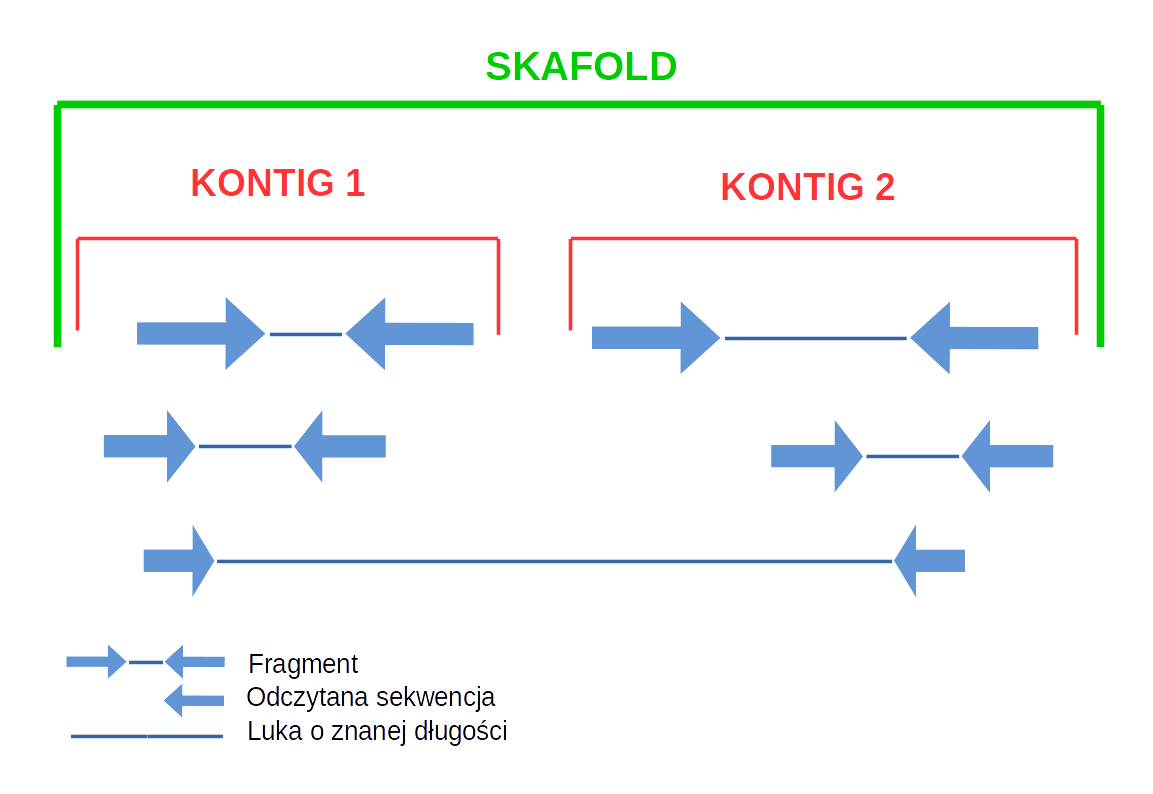
\includegraphics[width=0.8\textwidth]{grafika/contig_skafold.png}
%zdjecie przerobione z https://en.wikipedia.org/wiki/Contig#/media/File:PET_contig_scaffold.png
%https://upload.wikimedia.org/wikipedia/commons/6/6e/PET_contig_scaffold.png
\caption{Nakładające się zbiory sekwencji kontigów wraz z~lukami w~ujęciu skafoldu.}
\vspace{-0.8cm}
\caption*{\scriptsize Źródło: \url{https://upload.wikimedia.org/wikipedia/commons/6/6e/PET_contig_scaffold.png}}
\label{skafold_contig}
\end{figure}

\section{Historia}
Zalążki bioinformatyki sięgają lat osiemdziesiątych, kiedy to utworzono w~Stanach Zjednoczonych bazę danych \emph{GenBank}. Wraz z~coraz częstszymi badaniami różnych organizmów i~sekwencjonowaniem ich genomów przez badaczy, Amerykański Departament Energii zdecydował się na opracowanie ww. programu, aby gromadzić sekwencje DNA. %\cite{historia-bioinf}

Początkowo użytkownicy wprowadzali sekwencje DNA do systemu używając specjalnych klawiatur posiadających jedynie cztery klawisze - A, C, T oraz G. Z~biegiem czasu opracowano specjalne protokoły przekazywania danych, przyspieszające cały proces. Naukowcy mogli zadzwonić do \emph{GenBanku} i~używając komputera byli w~stanie bezpośrednio wprowadzić dane o~kolejnych fragmentach genomu do bazy (rys.\ref{historia-przeplywu-danych-sekwencji}). Rozwój technologii internetowych diametralnie zmienił sposób przekazywania informacji pomiędzy ośrodkami naukowymi. Po utworzeniu serwisu WWW, naukowcy z~całego świata otrzymali darmowy wgląd do zgromadzonych informacji. %\cite{historia-bioinf}

Zarząd \emph{GenBanku} przeniesiono do NCBI\footnote{National Center for Biotechnology Information} w~National Insitutes of~Health. Gdy wystartował Projekt Poznania Ludzkiego Genomu, ilość danych odbierana przez \emph{GenBank} rosła w~tempie wykładniczym. Wraz z~opracowaniem wydajnych metod sekwencjonowania wykorzystujących komputery, automatyczne sekwencjonery i~zagadnienia robotyki, proces gromadzenia danych niesamowicie przyspieszył. %\cite{historia-bioinf}

Równolegle prywatne firmy również zajęły się pokrewnymi badaniami tworząc własne ogromne zbiory danych. Aktualnie największe firmy potrafią w~krótkim odstępie czasu (1 dnia) zdekodować dane genetyczne liczące nawet kilkadziesiąt milionów par zasad DNA. Ilość danych jaką uzyskano z~pełnej sekwencji genomu ludzkiego to ponad 50~TB\footnote{Taka ilość danych zmieściłaby się na około 80 tys. płyt CD.} %\cite{historia-bioinf}
\begin{figure}[h]
\centering
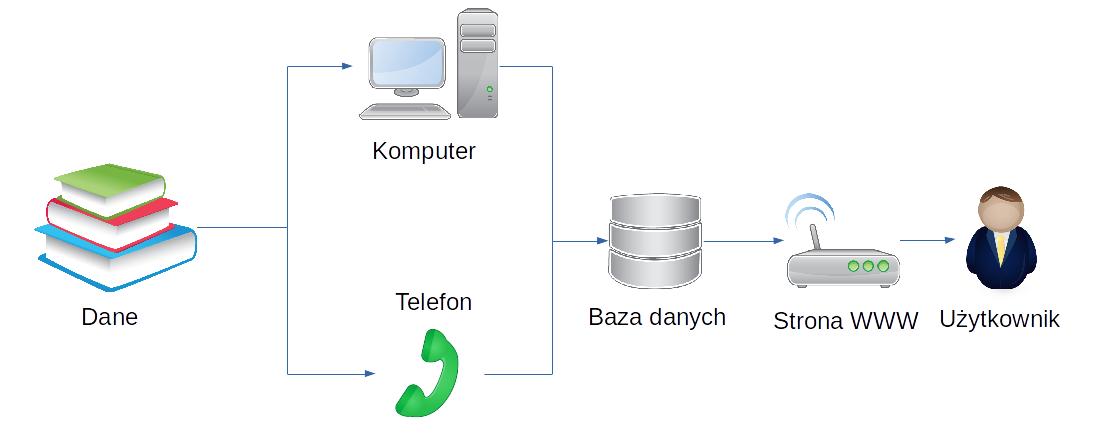
\includegraphics[width=0.9\textwidth]{grafika/historia.png}
%\renewcommand{\figurename}{Listing.}
\caption{Historyczny schemat przepływu informacji o~sekwencjach.}
\vspace{-0.8cm}
\caption*{\scriptsize Źródło: \url{http://www.uwm.edu.pl/wnz/KBZ/Lipazy/obrazy/his.gif}}
\label{historia-przeplywu-danych-sekwencji}
%http://www.uwm.edu.pl/wnz/KBZ/Lipazy/obrazy/his.gif
\end{figure}

\section{Oprogramowanie i~narzędzia}
Spektrum oprogramowania dostępnego dla bioinformatyki jest bardzo szerokie. Rozpoczyna się od prostych narzędzi z~interfejsem terminalowym, a~kończy na usługach internetowych i~złożonych programach z~możliwościami rozbudowanej interakcji z~użytkownikiem. %\cite{pl-wiki-bioinf}

Znaczna część narzędzi jest dostępna w~formie darmowej lub otwartego oprogramowania. Następstwem popytu na nowe algorytmy przeznaczone do analizy był dynamiczny rozwój nieodpłatnych programów. Dzięki ideologii otwartego kodu źródłowego, grupy badawcze z~całego świata mogą przyczynić się do tworzenia coraz to lepszych rozwiązań. Istotną zaletą darmowego oprogramowania jest budowanie standardów i~integrowanie bioinformatycznych informacji. %\cite{pl-wiki-bioinf}

\subsection{Bazy danych}
Bazy danych używane w~przeglądarkach genomów zwykle są ogromnymi zbiorami informacji, w~większości składającymi się z~sekwencji.Ponieważ bazy danych są niezbędnym elementem w~procesie badań naukowych, tworzenie ich jest jednym z~najistotniejszych zagadnień bioinformatyki. Dane przechowywane w~biologicznych bazach nie są niezmienne i~nieodwołalne. Wszystkie sekwencje są wynikiem badań o~określonej dokładności i~w konsekwencji nie można wykluczyć, że zbiór danych nie zawiera nieprawidłowości. %\cite{pl-wiki-bioinf}

Możliwość szybkiego i~precyzyjnego wyszukiwania pożądanych informacji jest jedną z~ważniejszych cech biologicznych baz danych. Najczęściej użytkownik oprócz obróbki danych ma również możliwość połączenia się przez internet z~innymi bazami. Charakteryzują się one zazwyczaj także małą redundancją danych. By ułatwić pracę, badacze często mają możliwość wyboru sposobu wyświetlania wyszukanych danych oraz wydruku, bądź ich zapisu. %\cite{pl-wiki-bioinf}

Pierwsze bazy danych zazwyczaj budowali biolodzy molekularni i~biochemicy. W~dzisiejszych czasach zwraca się uwagę, aby były one czytelne nie tylko dla specjalistów, ale i~dla badaczy z~nauk pokrewnych. %\cite{pl-wiki-bioinf}

\subsection{Usługi internetowe}
Dla wielu zastosowań bioinformatycznych zostały utworzone interfejsy wykorzystujące protokoły SOAP\footnote{Simple Object Access Protocol - protokół komunikacyjny, korzystający z~XML do kodowania wywołań. %\cite{pl-wiki-soap}
} i~REST\footnote{Representational State Transfer - styl architektury oprogramowania wywiedziony z~doświadczeń przy pisaniu specyfikacji protokołu HTTP dla systemów rozproszonych, wykorzystuje m.in. jednorodny interfejs oraz bezstanową komunikację. %\cite{pl-wiki-rest}
}. Dzięki takim rozwiązaniom, aplikacja działająca w~jednej części świata, potrafi korzystać z~algorytmów, danych i~mocy obliczeniowej serwerów podpiętych do sieci w~innych częściach globu. Brak obowiązku utrzymywania baz danych oraz zajmowania się oprogramowaniem stał się jednym z~największych udogodnień. Usługi bioinformatyczne zostały zgrupowane w~trzy podstawowe filary: dotyczące poszukiwania sekwencji, wielokrotnego przyrównywania sekwencji oraz analizy biologicznych sekwencji. Podział nastąpił z~inicjatywy Europejskiego Instytutu Informatyki (EBI). %\cite{pl-wiki-bioinf}

\section{Najpopularniejsze przeglądarki}
\subsection{Dostęp}
Obecnie dostępnych jest wiele przeglądarek. Dzięki ogólnoświatowej sieci komputerowej są szeroko używane przez badaczy. Czasem jednak możemy nie móc korzystać z~przeglądarek \emph{online}. Możliwe, że nie chcemy udostępniać danych innym użytkownikom, albo możemy dysponować zbyt dużą ich ilością, utrudniającą przesłanie na inny serwer. Rozwiązaniem problemu są przeglądarki \emph{offline} wyświetlające dane z~dysku, ale pobierające kontekst opisu genomu ze zdalnego serwera DAS\footnote{\emph{Distributed Annotation System} to protokół wymiany danych stworzony w~celu publikowania oraz integracji danych biologicznych, w~systemie rozproszonym. %\cite{pdf-mimuw}
}. %\cite{pdf-mimuw}
\subsection{Architektura}
Przeglądarki różnią się wewnętrzną organizacją. Jedne są scentralizowane, inne stawiają na rozproszony system przechowywania danych. Oba podejścia charakteryzują się wadami i~zaletami, w~zależności od rozpatrywanego punktu widzenia. Projekty zaprzęgające dużą część społeczności naukowej wymagają wysiłku od dużej liczby osób, często powodując wygasanie entuzjazmu w~pracy oraz wymagają praktycznie ciągłej aktualizacji. Specjalizowane bazy danych z~silną kuratelą %np.Swissprot
zmagają się niekiedy z~problemami finansowymi. Sprawowanie ciągłej kontroli nad systemem również opóźnia dostęp do danych. Praktyka pokazuje, że~tylko nieliczne bazy danych rozwijające się w~zamkniętych społecznościach mają szansę dobrze funkcjonować, co rzutuje na popularność użytkowania takich przeglądarek. Scentralizowane archiwa %(np.GenBank)
posiadają niekiedy niespójne albo wręcz żadne adnotacje\footnote{Adnotacja jest daną powiązaną z~jakimś elementem (np.sekwencją), dostarczającą nowych informacji na temat tego elementu - np. położenie eksonów, zawartość par GC, mutacje. %\cite{pdf-politech-poz}
} genomów. %\cite{pdf-politech-poz}

\subsection{Istniejące rozwiązania}
\begin{itemize}
\item \href{https://genome.ucsc.edu}{\emph{UCSC browser}} \label{UCSC}
autorstwa Jima Kenta, napisana w~większości w~języku~C w~2000~roku. Udostępniana darmowo dla akademickich zastosowań. Dla komercyjnych zastosowań wymagana licencja \emph{Kent Informatics}. %\cite{pdf-mimuw}

\item \href{http://gbrowse.org}{\emph{Gbrowse}} - \label{Gbrowse}
największa część kodu to Perl, z~czasem coraz więcej JavaScriptu. Prace rozpoczęto w~2002 roku, funkcjonuje na licencji \emph{PERL artistic license}. %\cite{pdf-mimuw}

\item \href{http://www.ensembl.org}{\emph{ENSEMBL}} \label{ENSEMBL}
- funkcjonuje na licencji Apache, dopuszczającej użycie kodu źródłowego zarówno na potrzeby wolnego oprogramowania, jak i~zamkniętego oprogramowania komercyjnego. Znaczna część kodu napisana w~Perlu, schemat bazy danych w~MySQl. %\cite{pdf-mimuw, pl-wiki-apache}

\item \href{http://bioviz.org/igb/index.html}{\emph{Integrated Genome Browser}} \label{IGB}
- projekt rozpoczęty przez firmę \emph{Affymetrix}, jednak porzucony przez nią i~rozwijany w~środowisku akademickim. Przeglądarka napisana w~Javie, obecnie na prawach Academic free license. %\cite{pdf-mimuw}
 
\item \href{http://www.interactive-biosoftware.com/alamut-visual/features/}{\emph{Alamut}} \label{alamut}- przeglądarka z~prostym interfejsem użytkownika z~adnotacjami pobieranymi z~publicznie dostępnych baz NCBI, EBI, UCSC. Zgodna z~nomenklaturą HGVS (ang. \emph{Human Genome Variation Society}). Funkcjonalność obliczeniowa oparta o~narzędzia predykcyjne.

\item \href{http://www.broadinstitute.org/annotation/argo/}{\emph{Argo Genome Browser}} \label{argo-genome-browser}- narzędzie służące do wizualizacji i~manualnego dodawania adnotacji genomów. Oprogramowanie open-source na licencji LGPL, napisane w~języku \emph{Java}.

\item \href{http://www.bioinformatics.babraham.ac.uk/projects/chipmonk/}{\emph{ChIPMonk}} \label{chipmonk}- narzędzie opracowane w~Instytucie Babraham Cambridge, służy do obrazowania i~analizy tablic danych \emph{ChIP-on-chip}. Kod wydany na licencji GPL v2. Projekt przestał być rozwijany.

\item \href{http://www.biodalliance.org/}{\emph{Biodalliance}} \label{biodalliance} - szybka, interaktywna wizualizacja genomów w~przeglądarce internetowej. Oparta o~\emph{JavaScript}, wspiera wiele najpopularniejszych formatów danych genetycznych. Rozwiązanie łatwe do wbudowania we własne aplikacje czy strony internetowe.

\item \href{https://www.dnanexus.com/genomes/hg18/public_browse}{\emph{DNAnexus}} \label{dnanexus} - przeglądarka do wizualizacji danych korzysta z~technologii \emph{Flash}. Jest narzędziem nowej generacji, mocno rozbudowanym w~kategorii analizy i~obrazowania sekwencji.

\item \href{http://download.cnet.com/GeneWall-Genome-Browser-Pro/3000-2129_4-75855506.html}{\emph{GeneWall}} \label{genewall} - przeglądarka genomów przeznaczona na urządzenia mobilne. W~wersji podstawowej można przeglądać jedynie genom człowieka, natomiast w~wariancie profesjonalnym aplikacji mamy możliwość uploadu własnych plików z~danymi.

\item \href{http://gaggle.systemsbiology.net/docs/geese/genomebrowser/}{\emph{Gaggle Genome Browser}} \label{gaggle} - otwarte narzędzie do mapowania mocno skondensowanych danych na współrzędne genomu. Oprogramowanie przeznaczone do obsługi dużych zbiorów danych, pozwala na łatwy import plików użytkownika. Współpracuje z~innymi bioinformatycznymi narzędziami zawartymi w~frameworku Gaggle.

\item \href{https://genestack.com/}{\emph{Genestack}} \label{genestack} - internetowy, genomiczny system operacyjny. Pozwala wyszukiwać i~importować dane z~wielu publicznych baz danych. Potrafi konwertować dane wejściowe użytkowników z~wielu formatów. Udostępnia zestaw narzędzi dla programistów, do łatwego tworzenia własnych przeglądarek.

\item \href{http://genomeview.org/}{\emph{GenomeView}} \label{genomeview} - samodzielna przeglądarka i~edytor genomu nowej generacji. Obecnie rozwijana przez społeczność \href{http://www.broadinstitute.org/}{Broad Insitute}. Zapewnia interaktywną wizualizację sekwencji, adnotacji, możliwość porównań na wielu poziomach, mapowań i~wielu innych. Dzięki systemowi wtyczek, istnieje możliwość rozszerzenia funkcjonalności przeglądarki.

\item \href{http://www.genomemaps.org/}{\emph{GenomeMaps}} \label{genomemaps} - wysokowydajna przeglądarka z~interfejsem opartym o~HTML5 i~CSS3. W~dużej mierze implementowana z~użyciem biblioteki Javascript \href{https://github.com/opencb/jsorolla}{\mbox{\emph{JSorolla}}}. Dane pozyskuje korzystając z~usług REST bazy \href{https://github.com/opencb/cellbase/wiki}{\emph{CellBase}}. Uruchamia się we wszystkich nowszych przeglądarkach internetowych, nie wymagając od użytkownika instalacji dodatkowych komponentów.

\item \href{http://www.popsci.com/science/article/2011-06/introducing-genome-wowser-ipad-app-lets-you-browse-human-genome}{\emph{Genome Wowser}} - aplikacja przeznaczona na urządzenia mobilne iPad, wydana przez CBMI (ang. Center for Biomedical Informatics) w~Szpitalu Dziecięcym w~Filadelfii. Pozwala przeglądać popularną bazę \emph{UCSC Genome Browser}.

\item \href{https://hyperbrowser.uio.no/hb/}{\emph{Genomic HyperBrowser}} - jest wolnym oprogramowaniem na licencji \emph{GNU GPL v3}. Produkt skupiony głownie na analizie statystycznej elementów w~genomie. Tworzony z~wykorzystaniem platformy \href{https://en.wikipedia.org/wiki/Galaxy_(computational_biology)}{\emph{Galaxy}}.

\item \href{http://wtsi-web.github.io/Genoverse/}{\emph{Genoverse}} - przenośna, konfigurowalna, przeglądarka oparta o~Javasript i~HTML5. Pozwala na eksplorację danych w~dynamiczny, interaktywny sposób. Dane są prezentowane w~przeglądarce, dzięki czemu może być łatwo instalowana na własnych stronach i~pokazywać dane z~wielu źródeł - gromadzonych online i~lokalnie.

\item \href{http://genplay.einstein.yu.edu/}{\emph{GenPlay}} - szybkie i~łatwe w~użyciu narzędzie do analizy i~przetwarzania sekwencji napisane w~Javie. Uruchamia się na większości najpopularniejszych systemów operacyjnych. Prace nad projektem rozpoczęto na Kolegium Medycznym Alberta Einstein'a Uniwersytetu Yeshiva w~Nowym Yorku. Przeglądarka aktualnie w~fazie testowania, używana przez studentów.

\item \href{http://img.jgi.doe.gov/}{\emph{Integrated Microbial Genomes}} - zaawansowany system wspierający analizę i~adnotacje mikrobiologicznych zbiorów danych i~metadanych genetycznych zgromadzonych w~\emph{DOE's Joint Genome Institute}. Współpracuje z~wieloma instytucjami.

\item \href{http://mgv2.cmbi.ru.nl/}{\emph{Microbial Genomic Viewer}} - łatwe w~obsłudze narzędzie do interaktywnej wizualizacji wyników analizy porównawczej genomów. 

\item \href{https://www.nextbio.com}{\emph{NextBio Genome Browser}} - interaktywna aplikacja pozwalająca na wizualizację zależności pomiędzy prywatnymi lub publicznymi zbiorami danych biologicznych różnych typów.

\item \href{http://persephone.net/}{\emph{Persephone}} - rozbudowana aplikacja nowej generacji szeroko używana przez bioinformatyków i~genetyków. Możliwość bezpłatnego korzystania z~wersji \emph{trial} przez 30 dni.

\item \href{http://www.plantgdb.org/}{\emph{PlantGDB}} - przeglądarka z~zestawem narzędzi analitycznych wraz ze zbiorami danych genetycznych wielu roślin.

\item \href{http://tabit.ucsd.edu/}{\emph{STAR}} - zintegrowane środowisko do zarządzania i~wizualizacji danych sekwencjonowania. Płynność działania aplikacji w~przeglądarce internetowej zapewnia połączenie technologi JavaScript, HTML5 i~asynchronicznej komunikacji do wymiany danych. 

\item \href{http://tgac-browser.tgac.ac.uk/}{\emph{TGAC Browser}} - nowa open-source'owa przeglądarka genomów obrazująca adnotacje z~bazy danych \emph{Ensembl}. Wyprodukowana przez \emph{Centrum Analizy Genomów} w~Wielkiej Brytanii (ang.\emph{The Genome Analysis Centre, UK}).

\item \href{http://ugene.net/}{\emph{Ugene}} - darmowa platforma bioinformatyczna wspomagająca użytkowników w~pracach nad sekwencjami. Oferuje narzędzia do analizy danych, przypisów, porównań itp. Dane wejściowe mogą być składowane lokalnie albo udostępnione z~innych źródeł. Napisana w~C++ z~wykorzystaniem biblioteki Qt. Funkcjonuje na licencji GPL.

\item \href{http://enhancer.lbl.gov/}{\emph{VISTA Enhancer Browser}} - kompleksowy zestaw baz danych, narzędzi, serwerów na potrzeby analizy porównawczej sekwencji genomów. Istnieją 2 sposoby na korzystanie z~przeglądarki: można wysyłać własne sekwencje i~dopasowania do analizy, bądź sprawdzać z~wstępnie przetworzonymi danymi całych genomów różnych gatunków. Projekt rozwijany we współpracy z~wieloma instytucjami.


\end{itemize}

\section{Porównanie}
Duża część z~dostępnych narzędzi oferujących gromadzenie danych sekwencji genomów to potężne platformy biologiczne oferujące funkcjonalność znacznie wykraczającą poza możliwości przechowywania i~wyświetlania danych sekwencji. Dostępne przeglądarki potrafią korzystać z~zewnętrznych, publicznie udostępnionych zbiorów danych w~celu przeprowadzania m.in. zaawansowanych analiz porównawczych wykorzystując różnego typu metadane i~adnotacje.
Aplikacja stworzona w~ramach przedmiotowej pracy inżynierskiej nie może konkurować z~innymi przeglądarkami genomów 
z kilku powodów.
Ważąca była niewątpliwie konieczność budowy oprogramowania samodzielnie i~w ograniczonym czasie. Wiele dostępnych aplikacji rozwijano w~ramach uczelni akademickich, angażując w~postęp rzesze naukowców z~różnych dziedzin. Mimo to, tworzenie tak rozbudowanych systemów zajmowało grupom co najmniej kilka lat.

Prezentowany w~przedmiotowej pracy system ma za zadanie umożliwić wysłanie i~przeglądanie danych zlokalizowanych na komputerze użytkownika, nie oferując przeprowadzania np. analiz statystycznych. Możliwe jest jedynie znakowanie wybranych odcinków sekwencji markerami.  

Prezentowana aplikacja wykazuje pewne podobieństwa do dostępnych przeglądarek pod względem zastosowanej architektury. Pomimo, że nie jest to reguła, coraz więcej podmiotów odpowiedzialnych za oprogramowanie decyduje się na rozwiązania oparte o~technologie uniezależniające końcowego użytkownika od posiadania konkretnej platformy sprzętowej. Technologie internetowe obsługiwane przez przeglądarki WWW wspierające HTML5 są rozwiązaniem zastosowanym również przez innych autorów.

Część dostępnych przeglądarek, tak jak w~przypadku prezentowanej aplikacji, jest tworzona w~postaci otwartego oprogramowania z~udostępnionym kodem źródłowym. Niektóre aplikacje są płatne, rozwijane przez prywatne firmy, zazwyczaj oferujące możliwość skorzystania z~bezpłatnego okresu próbnego w~celu przetestowania programu.


\chapter{Projekt i~implementacja}
Dane genetyczne przedstawiane są typowo w~postaci zbiorów łańcuchów znaków, gdzie każdy ciąg jest sekwencją symboli z~danego alfabetu. Reprezentacja łańcuchowa odzwierciedla fakt, że~kwasy nukleinowe (DNA i~RNA - cząsteczki przechowujące informacje genetyczne), są biopolimerami\footnote{Polimer występujący naturalnie w~organizmach żywych, produkowany przez nie.} 
nukleotydów\footnote{Podstawowy składnik strukturalny kwasów nukleinowych.}.
Kwasy nukleinowe odgrywają decydującą rolę jako nośnik informacji genetycznej nie tylko o~wszystkich elementach budowy organizmu ale również determinują jego rozwój i~funkcjonowanie. W~sekwencji nukleotydów nazwanej kodem genetycznym jest zakodowana informacja o~strukturze białek - zasadniczych składnikach struktur komórkowych oraz czynnikach przemian biochemicznych (enzymy, hormony). Białka zbudowane są z~aminokwasów połączonych wiązaniem peptydowym. 
Ustalono, że kod genetyczny jest:
\begin{itemize}
\item trójkowy, tzn, że jeden aminokwas jest zawsze kodowany przez trzy nukleotydy (kodon), 
\item nadmiarowy, tzn. że jeden aminokwas może być kodowany przez różne kodony
\item uniwersalny, tzn. że konkretny kodon odpowiada temu samemu aminokwasowi prawie u wszystkich gatunków
\item bezprzecinkowy, tzn. że pomiędzy nukleotydami w~kodzie genetycznym nie ma nukleotydów, które pełniłyby funkcję pauzy
\item niezachodzący, tzn. że nukleotydy konkretnego kodonu nie biorą udziału w~kodowaniu dwóch aminokwasów
\end{itemize}
 
Aplikacje wykorzystywane do analizy danych genetycznych, korzystają zazwyczaj z~ogromnych woluminów i~złożonych algorytmów. Wysoka wydajność, elastyczność oraz interfejs użytkownika z~wykorzystaniem przeglądarki internetowej to cechy aplikacji, które można osiągnąć łącząc ze sobą kilka języków programowania.
Różnorodność systemów i~użytkowników sprawia, że przenośność oprogramowania jest równie ważna. Badacze preferują korzystanie z~aktualizowanych automatycznie, graficznych interfejsów użytkownika dostępnych z~poziomu przeglądarek internetowych.

\section{Wymagania}
\begin{quote}
,,Wymaganiem jest każda właściwość oprogramowania potrzebna użytkownikowi do
zaspokojenia jego potrzeb. Wymaganiem jest każda właściwość oprogramowania
niezbędna do zatwierdzenia gotowego produktu. Wymaganiem jest każdy zapis dokumentujący właściwości określone w~dwóch poprzednich zdaniach.'' \cite{IEEE-wymagania} %\cite{inz-opr-k.sacha}%str.51
\end{quote}

Zacytowane słowa prezentują najistotniejsze idee inżynierii wymagań. Określić je można na wiele sposobów. Mogą różnić się zakresem którego dotyczą oraz poziomem szczegółowości. Wymagania najczęściej odnoszą się do różnych właściwości systemu i~zwyczajowo klasyfikujemy je na dwa sposoby:
\begin{itemize}
\item wymagania funkcjonalne
\item wymagania niefunkcjonalne
\end{itemize}

\subsection{Wymagania funkcjonalne}
Cechy systemu określane przez wymagania funkcjonalne, specyfikują zestaw funkcji realizowanych przez projektowany system:\\
\begin{itemize}
\item \textbf{Przeglądanie organizmów}\\
Użytkownik rozpoczynając używanie aplikacji ma możliwość wyboru organizmu będącego obiektem dalszej analizy. Prezentacja jest w~formie tabelarycznej.\\

\item \textbf{Przeglądanie chromosomów}\\
Materiał genetyczny organizmu zawarty jest w~zespole chromosomów. Użytkownik ma możliwość wyboru chromosomu danego organizmu. Widok jest w~formie graficznej oraz tabelarycznej.\\

\item \textbf{Przeglądanie skafoldów}\\
Jedną z~cech koniecznych do precyzyjnego i~szybkiego odszukiwania pożądanego fragmentu genomu jest możliwość nawigowania po genomie w~kontekście skafoldów, będących częścią informacji genetycznej zawartej w~chromosomie.\\

\item \textbf{Interaktywna nawigacja po sekwencji chromosomu}\\
Użytkownik może przeglądać dane sekwencji zawartej w~chromosomie w~formie interaktywnego widoku pozwalającego na:
\begin{itemize}
\item[$\bullet$] przybliżanie, oddalanie
\item[$\bullet$] przewijanie w~kierunku horyzontalnym
\item[$\bullet$] wprowadzenie granic wyświetlanego przedziału
\item[$\bullet$] wyświetlenie sekwencji ustalonego widoku
\end{itemize}
Dodatkowo system wyświetla podgląd informujący o~lokalizacji przeglądanego fragmentu genomu z~perspektywy całego chromosomu. Użytkownik ma do dyspozycji podziałkę z~jednostkami fizycznymi.
System umożliwia naniesienie na widok wybranych markerów przyporządkowanych do przeglądanego chromosomu.\\

\item \textbf{Dodawanie i~usuwanie organizmów}\\
Możliwość dodania do aplikacji nowego organizmu ze źródeł danych pozyskanych z~procesu sekwencjonowania genomu. Użytkownik ma możliwość usunięcia istniejącego organizmu z~aplikacji.
\end{itemize}

\subsection{Wymagania niefunkcjonalne}
Wymogi niefunkcjonalne inaczej znane jako wymagania jakościowe określają ograniczenia, przy zachowaniu których system powinien realizować swoje funkcje. Wymagania projektowanego systemu:

\begin{itemize}
\item \textbf{Wydajność oraz skalowalność}\\
System wspiera obsługę wielu połączonych użytkowników jednocześnie.
Ograniczenia czasowe uzależnione są głównie od posiadanego serwerowego sprzętu komputerowego. Maszyna kliencka nie musi być wysoce wydajna. System jest zdolny do zwiększenia wydajności poprzez dołączanie kolejnych zasobów do maszyny serwerowej.\\

\item \textbf{Połączenie z~siecią}\\
Projektowana aplikacja jest przystosowana do pracy w~sieci. Użytkownicy z~różnych maszyn wewnątrz sieci mają możliwość korzystania z~oprogramowania.\\

\item \textbf{Sprzęt komputerowy}\\
Do korzystania z~systemu konieczny jest komputer bądź inne urządzenie posiadające przeglądarkę internetową. Do uruchomienia części serwerowej aplikacji potrzebny komputer klasy PC.\\

\item \textbf{Oprogramowanie}\\
Przeglądarka internetowa użytkowników końcowych wspiera HTML5. Maszyna serwerowa posiada system operacyjny z~rodziny uniksopodobnych oparty na jądrze Linux.\\

\item \textbf{Przenośność}\\
Użytkownik ma możliwość korzystania z~aplikacji niezależnie od używanego systemu operacyjnego.\\

\item \textbf{Aktualizacja oprogramowania}\\
Wykonywanie aktualizacji oprogramowania wyłącznie po stronie serwera. Aktualne moduły klienckie ładowane podczas uruchomienia programu.


\end{itemize}

\section{Architektura}

Aplikacja została napisana w~oparciu o~architekturę wielowarstwową skupiającą się na odseparowaniu od siebie części programu pełniących różne role w~systemie. Takie podejście ułatwia pielęgnację kodu, dając możliwość modyfikacji poszczególnych warstw programu nie wpływając na inne. 

Jedną z~kluczowych cech wpływających na zdolność utrzymania dobrze zorganizowanego kodu jest jego czytelność. Programiści są zgodni, że model aplikacji trójwarstwowej ułatwia utrzymanie ,,czystego'' kodu.

Popularnym rozwiązaniem w~aplikacjach sieciowych jest koncepcja \emph{klient-serwer}, dzieląca program na część prezentacyjną, obsługującą dane oraz część odpowiadającą za logikę biznesową aplikacji.

Umiejscowienie modułów obliczeniowych po stronie serwera zwalnia klienta z~konieczności posiadania wydajnej maszyny, gdyż jego główne zadanie to prezentacja przetworzonych danych odebranych od serwera poprzez połączenie sieciowe. 
W dzisiejszych czasach praktycznie każda stacja robocza posiada jednostki obliczeniowe pozwalające na proste przetwarzanie. Sensownym podejściem wydaje się zrzucenie odpowiedzialności za operacje takie jak generowanie rysunków czy walidację danych na moduł klienta. Serwer musi być przystosowany do obsługi wielu klientów jednocześnie, zatem taka taktyka zmniejszy jego obciążenie do minimum. Rysunek \ref{klient-serwer} prezentuje rozmieszczenie poszczególnych modułów aplikacji.

\begin{figure}[h]
\centering
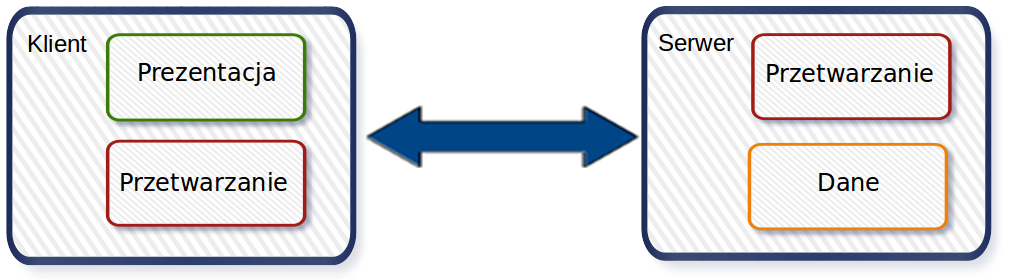
\includegraphics[width=1\textwidth]{grafika/klient_server/final_klient_serwer_poziomo.png}
\caption{Model aplikacji trójwarstwowej projektowanego systemu.}
\vspace{-0.8cm}
\caption*{\scriptsize Źródło: \url{http://www.hindawi.com/journals/bmri/2014/253013/fig1/}}
\label{klient-serwer}
\end{figure}

Oprogramowanie zostało zbudowane w~oparciu o~framework \emph{bioweb}\footnote{\url{http://bioweb.sourceforge.net/pl/index.html}} przystosowany do tworzenia aplikacji operujących na danych genetycznych. Łączy ze sobą wiele technologii, korzystając z~zalet języków kompilowanych i~interpretowanych. Rysunek \ref{ogolny_schemat} przedstawia ogólny schemat projektowanej aplikacji z~uwzględnieniem zastosowanych narzędzi.

%Wyizolowane składniki systemu, mogą być rozmieszczone na różnych maszynach, jednakże trzeba opracować odpowiednie interfejsy pozwalające na komunikację między modułami.
%Baza danych została umiejscowiona po stronie serwera, zwiększając tym samym bezpieczeństwo danych.
%-------------------------
%Jednym z celów budowania systemów klient-serwer, jest umożliwienie dostępu do danych, niezależnie od lokalizacji serwera. Projektowana aplikacja do tego celu korzysta z połączenia sieciowego.
%Część związana z realizacją biznesowych usług systemu znajduje się na wydajnej maszynie serwerowej, uniezależniając klienta od konieczności posiadania szybkiego sprzętu. Zadaniem klienta jest




\begin{figure}[h]
\centering
%http://bioweb.sourceforge.net/architecture.png
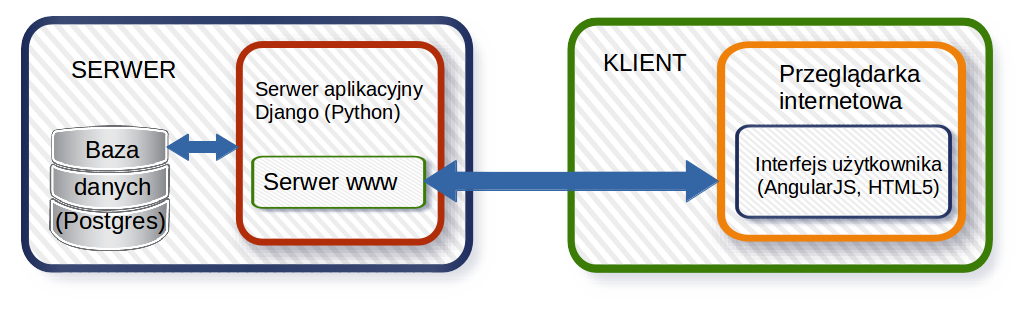
\includegraphics[width=1\textwidth]{grafika/ogolny_schemat.png}
\caption{Schemat struktury projektowanej aplikacji.}
\vspace{-0.8cm}
\caption*{\scriptsize Źródło: \url{http://bioweb.sourceforge.net/architecture.png}}
\label{ogolny_schemat}
\end{figure}
\section{Warstwa trwałości}
Do prawidłowego i~efektywnego funkcjonowania aplikacji potrzebna jest możliwość gromadzenia danych cyfrowych zgodnie z~przyjętymi zasadami wynikającymi z~analizy wymagań. Warstwa danych składuje stan aplikacji, umożliwiając jego odczyt i~modyfikację. Operacje modyfikujące dane składające się z~wielu elementarnych operacji powinny być przeprowadzane wszystkie jako całość albo wcale. Pożądaną cechą tej warstwy jest możliwość obsługi nowych żądań, bądź zgłaszania niepowodzenia odczytu lub zapisu, podczas obsługi aktualnych żądań. Na tym poziomie najczęściej korzysta się z~gotowych, zaimplementowanych już systemów bazodanowych lub systemów plików.  %\cite{it-pwn}

\subsection{PostgreSQL}
Wykorzystanym systemem bazodanowym w~pracy jest \emph{PostgreSQL} (zwany \emph{Postgres}). Jest to potężny obiektowo-relacyjny system open source, z~historią ponad 15 lat aktywnego rozwoju. Wypracował silną reputację niezawodności, spójności danych i~poprawności. Działa na większości systemów operacyjnych takich jak \emph{UNIX, Mac OS X} czy \emph{Windows}.

\subsection{ORM}
\emph{Django} dostarcza maper obiektowo relacyjny (ang. \emph{Object Relational Mapping}) pozwalający operować na zgromadzonych danych, praktycznie bez potrzeby wykorzystywania języka \emph{SQL}, jednak nie wykluczający takiej możliwości. Bogate API umożliwia przeprowadzanie nawet mocno skomplikowanych zapytań w~stosunkowo prosty sposób. Często przy korzystaniu z~ORM pojawiają się liczne problemy wydajnościowe jednak w~omawianym projekcie nie sprawiły one problemu. Korzystanie z~mapera okazało się wygodne i~dość intuicyjne, jednocześnie będąc mało podatnym na popełnianie błędów przez programistę.

\section{Warstwa przetwarzania}
W~niniejszym podrozdziale omawiam narzędzia i~technologie programistyczne, użyte w~pracy na poziomie warstwy przetwarzania. Warstwa ta odpowiada za logikę biznesową i~wykonywane operacje w~systemie. Pełni rolę kontrolera - komunikuje się z~warstwą danych i~prezentacji, koordynując pracę nad całością systemu. Jej głównym zadaniem jest przetwarzanie żądań przychodzących od klientów i~zwrócenie im oczekiwanej odpowiedzi. Odpowiedni dobór narzędzi może w~znacznym stopniu uprościć i~przyspieszyć proces wytwarzania oprogramowania.

\subsection{Python}
\emph{Python} to język programowania wysokiego poziomu, który łączy w~sobie zalety tradycyjnych języków, takich jak \emph{C/C++} i~\emph{Java}, z~łatwością i~szybkością tworzenia aplikacji w~językach skryptowych, takich jak \emph{Ruby} czy \emph{VBScript}. Daje to jego użytkownikom możliwość tworzenia aplikacji, które mogą rozwiązywać różnorodne problemy. %\cite{python_i_django}

\begin{figure}[h]
\centering
%http://www.zerothtech.com/image/page3/python.png

\includegraphics[width=1\textwidth/2]{grafika/loga/python.png}
\caption{Logo języka programowania \emph{Python}}
\vspace{-0.8cm}
\caption*{\scriptsize Źródło: \url{http://www.zerothtech.com/image/page3/python.png}}
\label{logo_python}
\end{figure}

Przyglądając się logo języka (Rys.\ref{logo_python}), można przypuszczać, że nazwa języka pochodzi od zwierzęcia - gatunku węża. Nic bardziej mylnego. Twórca \emph{Pythona} - holenderski programista Guido van Rossum, był fanem serialu komediowego ,,Latający Cyrk Monty Pythona'' (ang. \emph{,,Monty Python's Flying Circus''}), który emitowano w~latach siedemdziesiątych przez głównego brytyjskiego publicznego nadawce radiowo-telewizyjnego BBC. %\cite{python_i_django} %wikipedia python

\emph{Python} realizuje kilka paradygmatów programowania, pozwalając programiście na stosowanie jednocześnie. Wspiera programowanie obiektowe, strukturalne oraz funkcyjne. W~celu zarządzania dynamicznie przydzieloną pamięcią używa metod automatycznego zbierania nieużytków (ang. \emph{garbage collection}).

Zaletą \emph{Pythona} jest jego liczna społeczność. Posiada bardzo dużą liczbę użytkowników\footnote{Według autora książki \emph{Learning Python 5th Edition}, w~2013 roku było mniej więcej milion użytkowników \emph{Pythona}.\cite{learning-python}}, co ułatwia często rozwiązywanie napotykanych problemów. Istnieje bowiem spora szansa na to, że już ktoś kiedyś miał ten sam problem co my i~pomocne informacje zmieścił w~sieci.

Powodem użycia tego języka, oprócz wspomnianej popularności jest:
\begin{itemize}
\item \textbf{Jakość oprogramowania}\\
Dla wielu, jedną z~najważniejszych cech \emph{Pythona} jest jego spójność i~wysoka ogólna jakość. Kod ma być czytelny i~prosty w~utrzymaniu, o~wiele prostszy od tradycyjnych języków skryptowych. Uniformizm sprawia że jest łatwy do zrozumienia. \emph{Python} ma głębokie wsparcie dla bardziej zaawansowanych mechanizmów ponownego użycia takich jak programowanie funkcyjne czy programowanie zorientowane obiektowo.

\item \textbf{Efektywnosć pracy}\\
Stosowanie \emph{Pythona} przyspiesza proces wytwarzania oprogramowania wiele razy w~porównaniu do statycznie typowanych języków takich jak \emph{C, C++} czy \emph{Java}. Kod zajmuje zazwyczaj od jednej trzeciej do jednej piątej rozmiaru kodu napisanego w~innym języku kompilowanym. Oznacza to, że jest mniej do pisania, mniej do debugowania, a~także mniej do utrzymywania. Programy tworzone w~\emph{Pythonie} uruchamiają się natychmiast, bez długich kompilacji i~nie wymagają kroków takich jak np. linkowanie.

\item \textbf{Przenośność programów}\\
Większość programów napisanych w~\emph{Pythonie} można uruchomić bez zmian na wszystkich najpopularniejszych platformach komputerowych. Przenoszenie kodu pomiędzy \emph{Linuxem} a~\emph{Windowsem} polega zwykle na po prostu skopiowaniu plików programu pomiędzy maszynami. \emph{Python} oferuje wiele opcji do implementacji przenośnych graficznych interfejsów, aplikacji webowych czy też programów łączących się z~bazami danych. W~dużej mierze wspierane są nawet operacje korzystające z~interfejsów systemów operacyjnych, takie jak uruchamianie procesów czy działania na lokalnym systemie plików w~ujednolicony dla użytkownika sposób.

\item \textbf{Biblioteki}\\
Rozpoczynając użytkowanie \emph{Pythona} dostajemy na starcie zbiór sporej biblioteki standardowej oferującej przenośną funkcjonalność. Ta biblioteka wspiera szereg zadań programistycznych na poziomie aplikacji - od dopasowywania wzorców regularnych do eleganckich rozwiązań sieciowych. Firmy trzecie oferują mocno rozbudowane narzędzia do budowy stron internetowych, rozwoju gier i~wiele innych. Dla przykładu - rozszerzenie \emph{NumPy} zostało niejednokrotnie określone mocniejszym rozwiązaniem od \emph{Matlaba} (w dodatku darmowym) w~kontekście programowania numerycznego.

\item \textbf{Integracja z~komponentami}\\
Skrypty \emph{Pythona} z~łatwością mogą komunikować się z~innymi częściami aplikacji za pomocą różnorodnych mechanizmów integracyjnych. Takie integracje pozwalają na wywoływanie wewnątrz kodu \emph{Pythona}, instrukcji napisanych w~\emph{C}, bądź \emph{C++}. Potrafimy korzystać z~skryptów też analogicznie w~drugą stronę (wykonanie kodu \emph{Pythona} wewnątrz np. \emph{C++}). Współpraca z~fragmentami aplikacji napisanymi w~\emph{Javie} czy komponentami \emph{.NET} również jest możliwa. \emph{Python} potrafi współdziałać z~urządzeniami poprzez COM (ang. \emph{Component Object Model}), porty szeregowe czy interfejsy sieciowe takie jak \emph{SOAP} czy \emph{CORBA}.

\item \textbf{Frajda}\\
Ze względu na łatwość obsługi i~zestaw wbudowanych narzędzi, \emph{Python} może wnieść do programowania więcej przyjemności niż przykrych obowiązków. Pomimo, że są to korzyści niematerialne, ich wpływ na produktywność jest dość ważnym atutem.

\end{itemize}

Bardzo pomocny w~pisaniu pracy okazał się interaktywny interpreter \emph{Pythona}. Pozwala on na m.in. testowanie linijek kodu bez konieczności tworzenia, edycji i~uruchamiania źródłowego pliku. Powłoka języka nie tylko sprawdza poprawność napisanego kodu, ale także pozwala wykorzystać inne funkcje związane z~pracą z~kodem, jak np. sprawdzanie struktur danych. Doceniając zalety idei interaktywnego interpretera warto zaznajomić się z~narzędziem \emph{IPython}. Od tradycyjnego interpretera różni się zakresem możliwości - oferuje dodatkowo takie cechy jak: %\cite{python_i_django}
\begin{itemize}
\item dostęp do powłoki systemowej
\item numerowanie linii
\item automatyczne wcięcia
\item historię poleceń
\item profilowanie kodu pod względem wydajności i~zajętości pamięci.
\end{itemize}

\subsection{Django}
Każdy programista tworząc aplikację internetową zmaga się z~takimi samymi trudnościami na pewnych etapach tworzenia oprogramowania. Ludzie projektują frameworki webowe, aby zautomatyzować czynności powtarzające się przy projektowaniu stron internetowych, dzięki czemu możemy się skupić na pisaniu aplikacji bez konieczności ,,wymyślania koła na nowo''. Jednym z~nich jest właśnie \emph{Django}. %\cite{django-girls, django}
\begin{figure}[h]
\centering

\includegraphics[width=1\textwidth/3]{grafika/loga/django.png}
\caption{Logo frameworku \emph{Django}.}
\vspace{-0.8cm}
\caption*{\scriptsize Źródło: \url{http://www.slothparadise.com/wp-content/uploads/2014/11/django.png}}
\label{logo_django}
%http://www.slothparadise.com/wp-content/uploads/2014/11/django.png
\end{figure}

\emph{Django} jest w~pełni darmowym, open-source'owym projektem rozpoczętym w~2003 roku, napisanym w~całości w~Pythonie. Nazwa frameworku pochodzi od imienia jednego z~najwybitniejszych gitarzystów wszech czasów - francuza Django Reinhardta. Jest prosty, ale i~elastyczny zarazem, dzięki czemu pozwala na projektowanie różnorodnych rozwiązań bez niepotrzebnych kosztów za pomocą względnie niedużej ilości kodu.

\subsubsection{Sposób działania}
W momencie gdy serwer otrzymuje żądanie, dostarcza je do \emph{Django}, aby ten wywnioskował do czego się odnosi. Framework weryfikuje początkowo adres strony i~uzgadnia co robić dalej. Modułem odpowiedzialnym za sprawdzenie adresu jest \emph{urlresolver}. Jego działanie nie jest zbyt skomplikowane, bowiem sprowadza się do odnalezienia wzorca regularnego pasującego do adresu URL. Gdy odnajdzie pierwszy pasujący wzorzec przekazuje żądanie dalej, do stosownej funkcji nazywanej \emph{widokiem}. %\cite{django-girls}

W funkcjach widoków implementowana jest logika biznesowa przetwarzająca żądanie i~generująca odpowiedź (ang. \emph{response}). Na tym etapie następuje najczęściej interakcja z~bazą danych poprzez ORM, obejmująca operacje takie jak wyszukiwanie oraz modyfikacje rekordów danych zawartych w~warstwie danych aplikacji. Wyprodukowaną odpowiedź \emph{Django} wysyła do przeglądarki użytkownika. Uproszczony schemat działania ilustruje rysunek.\ref{schemat_django}

\begin{figure}[h]
\centering
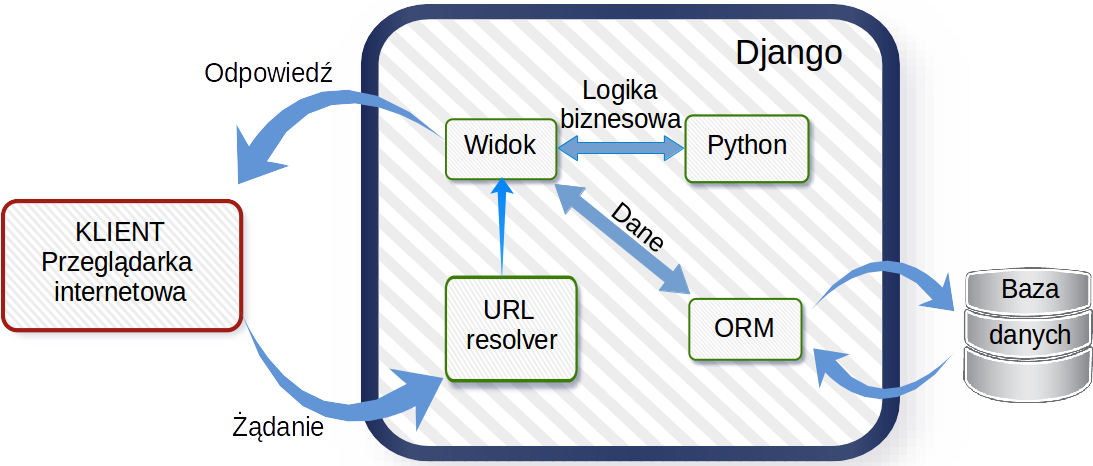
\includegraphics[width=1\textwidth]{grafika/schemat_django.png}
\caption{Schemat ilustrujący w~uproszczeniu sposób funkcjonowania \emph{Django}.}
\label{schemat_django}
%http://www.slothparadise.com/wp-content/uploads/2014/11/django.png
\end{figure}

\subsection{Gunicorn}
Zalecanym przez twórców \emph{Django} sposobem na wdrożenie aplikacji opartej o~ich autorski framework, jest skorzystanie z~WSGI (ang. \emph{Web Server Gateway Interface}). Aplikacje internetowe napisane w~języku \emph{Python} projektowane były najczęściej pod kątem jednego z~pośród wielu interfejsów do komunikacji z~serwerem www. Często miały problem ze współpracą z~ww. serwerami i~vice versa. WSGI został stworzony jako interfejs niskiego poziomu w~komunikacji między nimi w~celu promowania wspólnej podstawy dla rozwoju przenośnych aplikacji internetowych napisanych z~użyciem Pythona. %\cite{en-wiki-wsgi}
\begin{figure}[h]
\centering

\includegraphics[width=1\textwidth/(25/10)]{grafika/loga/gunicorn.png}
\caption{Logo serwera \emph{Gunicorn}.}
\vspace{-0.8cm}
\caption*{\scriptsize Źródło: \url{http://gunicorn.org/images/large_gunicorn.png}}
\label{logo_gunicorn}
%http://gunicorn.org/images/large_gunicorn.png
\end{figure}

\emph{Gunicorn}\footnote{Green Unicorn} jest serwerem HTTP implementującym interfejs WSGI dla systemu UNIX. Jest bliźniaczym oprogramowaniem przeniesionym z~projektu \emph{Unicorn} skierowanego dla języka \emph{Ruby}. Serwer \emph{Gunicorn} jest kompatybilny z~szeroką gamą frameworków internetowych. Podczas działania używa niewielkiej ilości zasobów oraz jest dość szybki, co czyni go niewątpliwie atrakcyjnym rozwiązaniem. %\cite{gunicorn}
\subsection{Nginx}
%grafika nginx - https://assets.wp.nginx.com/wp-content/uploads/2015/04/NGINX_logo_rgb-01.png
W środowisku produkcyjnym projektowana aplikacja korzysta z~\emph{Nginx}.
\emph{Nginx} jest serwerem WWW oraz serwerem proxy dla HTTP i~IMAP/POP3. Twórcą jest Igor Sysojew. Dzięki swojej niezawodności, wysokiej wydajności i~możliwości prostej, wysoce elastycznej konfiguracji, zyskał uznanie na całym świecie. Obecnie znajduje się na liście wśród 3 najczęściej używanych serwerów WWW, konkurując z~serwerem \emph{Apache} czy produktami \emph{Microsoftu}. %\cite{nginx}
\begin{figure}[h]
\centering
%http://logonoid.com/images/nginx-logo.png

\includegraphics[width=1\textwidth/3]{grafika/loga/nginx.png}
\caption{Logo serwera Nginx.}
\vspace{-0.8cm}
\caption*{\scriptsize Źródło: \url{http://logonoid.com/images/nginx-logo.png}}
\label{logo_nginx}
\end{figure}

Zaprojektowany został by stawić czoło problemowi \emph{C10K}, polegającemu na obsłużeniu 10 tysięcy użytkowników jednocześnie. W~przeciwieństwie do tradycyjnej architektury serwerów, \emph{Nginx} do obsługi żądań nie używa osobnych wątków. Wykorzystuje architekturę sterowaną zdarzeniami. Dzięki asynchorniczności, nawet w~trakcie dużego obciążenia korzysta z~relatywnie małych przewidywanych ilości pamięci. %\cite{nginx}

\begin{figure}[h]
\centering
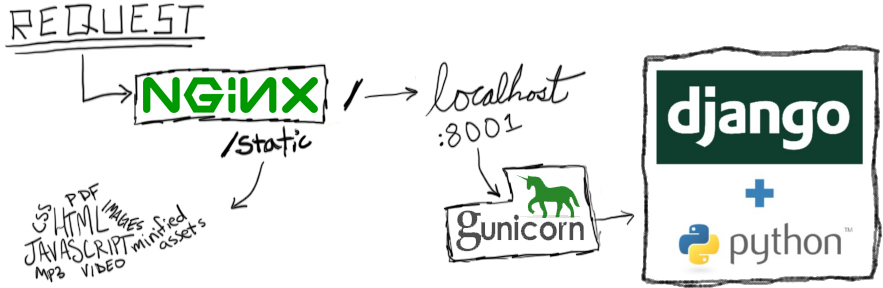
\includegraphics[width=1\textwidth]{grafika/nginx_gunicorn_flask/nginx-gunicorn-django.png}
\caption{Schemat prezentujący przepływ żądania http w~warstwie przetwarzania.}
\vspace{-0.8cm}
\caption*{\scriptsize Źródło: \url{https://raw.githubusercontent.com/realpython/flask-deploy/master/images/localhost2.jpg}}
\label{nginx-gunicorn-django}
%https://raw.githubusercontent.com/realpython/flask-deploy/master/images/localhost2.jpg
\end{figure}

\section{Warstwa prezentacji}
Zadaniem warstwy prezentacji jest pobieranie żądań od użytkownika oraz wizualizacja wyników przetwarzania. Zasadniczą czynnością, którą wykonuje jest konwersja danych z~postaci akceptowalnej przez system do formy czytelnej dla człowieka i~odwrotnie. W~przypadku zastosowania graficznego interfejsu użytkownika (ang. \emph{graphical user interface - GUI}), warstwa ta monitoruje i~interpretuje stan urządzeń wskazujących oraz dostarcza właściwych elementów graficznych.

\subsection{HTML5}
Jest to język, który został opracowany głównie w~celu tworzenia i~prezentowania internetowych stron www. Jest kolejną wersją języka HTML, w~której kładziono nacisk na m.in. wprowadzenie nowych elementów zwiększających możliwości interaktywne i~multimedialne prezentowanych treści.
\begin{figure}[h]
\centering

\includegraphics[width=0.3\textwidth]{grafika/loga/HTML5.png}
\caption{Logo języka HTML5.}
\vspace{-0.8cm}
\caption*{\scriptsize Źródło: \url{https://www.w3.org/html/logo/downloads/HTML5_Logo_512.png}}
\label{html5}
%https://www.w3.org/html/logo/downloads/HTML5_Logo_512.png
\end{figure}

\subsubsection{Canvas}
Jedną z~nowinek jakie wprowadzono w~HTML5 jest element \emph{Canvas}. Pozwala na dynamiczne rysowanie grafik 2D i~3D przy pomocy zazwyczaj Javascriptowych skryptów bez konieczności instalacji dodatkowych wtyczek. W~projektowanej przeze mnie przeglądarce stanowi istotny element, będący główną częścią widoku w~graficznym interfejsie użytkownika.
\subsection{JavaScript}
Do wprowadzenia interaktywności na stronie korzystam z~\emph{JavaScriptu}. Umożliwia modyfikowanie zawartości kodu znaczników stron, za pomocą których strony te mogą być wyświetlane w~przeglądarkach www. Cennym zastosowaniem jest dodanie przetwarzania po stronie klienta, nie wymagającego logiki serwera. Zdolność dynamicznego reagowania na zdarzenia użytkownika polepsza ogólne odczucia końcowego odbiorcy, czyniąc aplikację bardziej atrakcyjną. %\cite{javascript}
\subsection{AngularJS}
Angular to framework Javasciptowy wzbogacający kod HTML przetwarzany przez przeglądarkę internetową. Dostarcza podstawy ułatwiające tworzenie rozbudowanych, bogatych aplikacji internetowych opartych o~wzorzec projektowy MVC (ang. \emph{Model-View-Controller}).
Stosowanie go w~projektach upraszcza organizacje kodu, sprawia że oprogramowanie staje się łatwe w~konserwacji i~rozbudowie.
Angular jest biblioteką typu open source, sponsorowaną i~rozwijaną przez \emph{Google}. Zastosowanie znajduje w~największych i~najbardziej skomplikowanych programach sieciowych ale również doskonale się spisał przy implementacji aplikacji będącej przedmiotem pracy inżynierskiej. %\cite{angular}
\begin{figure}[h]
\centering

\includegraphics[width=0.7\textwidth]{grafika/loga/angular.png}
\caption{Logo frameworku AngularJS.}
\vspace{-0.8cm}
\caption*{\scriptsize Źródło: \url{https://angularjs.org/img/AngularJS-large.png}}
\label{angular}
%https://angularjs.org/img/AngularJS-large.png
\end{figure}

\subsection{Bootstrap}
Stworzenie profesjonalnej, nowoczesnej strony internetowej od zera wymaga dużo czasu i~wysiłku od programisty. Dzisiejsze strony powinny działać szybko, być eleganckie i~elastyczne. W~dobie urządzeń mobilnych, coraz częściej wymaga się aby i~na nich aplikacje poprawnie działały. Cytując autora książki wprowadzającej w~świat Bootstrapa:
\begin{quote}
,,Bootstrap ułatwia projektantom i~programistom
pracę, oferując szeroką gamę gotowych komponentów HTML oraz elastyczną strukturę
w postaci systemu siatkowego, dzięki którym tworzenie profesjonalnych, responsywnych
szablonów stron internetowych jest bardzo proste i~trwa zdecydowanie krócej niż w~przypadku tradycyjnych rozwiązań.'' \cite{bootstrap}
\end{quote}
Bootstrap okazał się bardzo użyteczny przy implementacji elementów graficznych, nadając im elegancki wygląd i~miejscami ożywiając je płynnymi animacjami. Próba tworzenia samodzielnie takich komponentów zajęłaby zdecydowanie zbyt wiele czasu.

\begin{figure}[h]
\centering

\includegraphics[width=0.6\textwidth]{grafika/loga/bootstrap.png}
\caption{Logo frameworku Bootstrap.}
\vspace{-0.8cm}
\caption*{\scriptsize Źródło: \url{http://shoplivechat.com/wp-content/uploads/2014/08/tech_bootstrap.png}}
\label{bootstrap}
%http://shoplivechat.com/wp-content/uploads/2014/08/tech_bootstrap.png
\end{figure}

\section{Inne narzędzia}
\subsection{Zintegrowane środowisko programistyczne}
% grafika pycharm - http://img.darktorrent.pl/vNRMIF2.gif
Zastosowanie aplikacji IDE (ang. \emph{Integrated Development Enviroment}) ułatwia i~przyspiesza proces tworzenia kodu m.in. na etapach takich jak modyfikowanie, testowanie oraz konserwowanie oprogramowania. Programy będące zintegrowanymi środowiskami programistycznymi oferują złożoną, wieloaspektową funkcjonalność wspierającą programistę w~wielu czynnościach. Omawiane aplikacje pomagają na poziomach:
\begin{itemize}
\item edycji i~analizy kodu źródłowego
\item kompilacji kodu źródłowego
\item debugowania
\item testowania
\item refaktoryzacji kodu źródłowego
\item tworzenia zasobów programu takich jak elementy graficzne, ikony, obrazy itd.
\item tworzenia baz danych, komponentów.
\end{itemize}

Używanym przeze mnie środowiskiem jest produkt \emph{PyCharm} firmy \emph{JetBrains}. Posiada wszystkie cechy profesjonalnego narzędzia programistycznego. Jednym z~powodów motywujących mnie do wyboru tego środowiska był fakt, że wspiera wiele frameworków, w~tym użytych przeze mnie \emph{Django} oraz \emph{AngularJS}. %\cite{pycharm}
\begin{figure}[h]
\centering

\includegraphics[width=1\textwidth/2]{grafika/loga/jetbrains_pycharm_pionowo.png}
\caption{Logo firmy JetBrains i~zintegrowanego środowiska programistycznego PyCharm.}
\vspace{-0.8cm}
\caption*{\scriptsize \hspace{-5.2cm} Źródła: \url{http://away3d.com/images/carousel/logo_jetbrains.png}}
\vspace{-0.8cm}
\caption*{\scriptsize \url{http://blog.pirx.ru/media/files/2015/type-hinting-talk/media/pycharm-logo.png}}
\label{logo_jetbrains_pycharm}
%grafika pycharm - http://blog.pirx.ru/media/files/2015/type-hinting-talk/media/pycharm-logo.png
%grafika jetbrains - http://away3d.com/images/carousel/logo_jetbrains.png
\end{figure}

Oferowana spora liczba wtyczek pozwala znacznie rozszerzyć możliwości aplikacji. Ciekawą funkcjonalnością okazała się możliwość instalacji wtyczki do \emph{Google Chrome} pozwalającej na debugowanie kodu JavaScript w~przeglądarce internetowej, sterując sesją bezpośrednio z~oprogramowania \emph{JetBrains}. W~trakcie debugowania \emph{PyCharm} wspiera również edytowanie kodu HTML i~CSS ,,na żywo'', utrzymując aktualny obiektowy model dokumentu - DOM (ang. \emph{Dokument Object Model}).

Używałem środowiska w~wydaniu 5-tym \emph{Professional Edition}, dzięki czemu mogłem korzystać z~pełnej wersji programu. Możliwość bezpłatnego użytkowania uzyskałem na podstawie licencji studenckiej.

\subsection{System kontroli wersji}
System kontroli wersji\footnote{Inaczej system kontroli rewizji (ang.\emph{revision control system}).} to narzędzie pozwalające kontrolować zmiany przeprowadzane na plikach. W~dowolnej chwili umożliwia odtworzenie którejkolwiek z~wcześniejszych wersji projektu. Narzędzie pozwala na łatwy nadzór pracy nad projektem wykonywanym przez kilka osób. Podstawowe możliwości jakie oferuje użytkownikom to m.in.: %\cite{git}
\begin{itemize}
\item przywrócenie plików do poprzedniej wersji
\item odtworzenie stanu całego projektu
\item porównywanie wprowadzonych zmian
\item dowiedzenie się kto i~kiedy modyfikował dany fragment projektu.
\end{itemize}

Zastosowanie narzędzia sprawia, że nawet jeśli zostanie popełniony błąd, bądź dane zostaną utracone, w~stosunkowo łatwy sposób można przywrócić stan projektu do pożądanej formy. %\cite{git}

Ze względu na dynamicznie rosnącą popularność w~ostatnich latach, zdecydowałem się skorzystać z~rozproszonego systemu kontroli rewizji \emph{Git}. W~celu ułatwienia koordynacji pracy, repozytorium zostało umieszczone w~serwisie \emph{GitHub}. Jest to jedno z~najbardziej popularnych rozwiązań hostingowych projektów open source. Piki repozytorium projektu znajdują się pod adresem: %\cite{git}
\begin{center}
\url{https://github.com/mhaponiu/przegladarkaGenomow.git}
\end{center}

\begin{figure}[]
\centering

\includegraphics[width=1\textwidth/2]{grafika/loga/git_github_pionowo.png}
\caption{Logo systemu kontroli wersji \emph{Git} i~serwisu hostingowego \emph{GitHub}.}
\vspace{-0.8cm}
\caption*{\scriptsize \hspace{-4.7cm} Źródła: \url{https://git-scm.com/images/logo@2x.png}}
\vspace{-0.8cm}
\caption*{\scriptsize \url{http://lumiinsight.com/wp-content/uploads/2015/11/GitHub.jpg}}
\label{logo_git_github}
%grafika git - https://git-scm.com/images/logo@2x.png
%grafika github - http://lumiinsight.com/wp-content/uploads/2015/11/GitHub.jpg
\end{figure}

W~trakcie trwania projektu wykonałem 105 commitów.

\section{Szczegóły implementacyjne}

Szacuję, że implementacja programu wymagała około 600 roboczo godzin.
Łącznie napisałem ponad 4 tysiące linii kodu, przy czym wykonanie poszczególnych warstw przetwarzania i prezentacji zajęły odpowiednio: 2500~i 1600 linii kodu.

\subsection{Dane}
Struktura danych została tak zaprojektowana aby umożliwiała przechowywanie informacji o~organizmach, chromosomach, skafoldach, sekwencjach, markerach i~ich znaczeniach, możliwie dokładnie oddając ich naturę.

Baza została wygenerowana przez \emph{Django} z~wykorzystaniem \emph{mapera obiektowo relacyjnego} (ORM) na podstawie przygotowanych klas znajdujących się w~pliku \emph{models.py}. Diagram klas przedstawiający strukturę obiektową został pokazany na rys.\ref{diagram_klas_modelu}.
\begin{figure}[b]
\centering
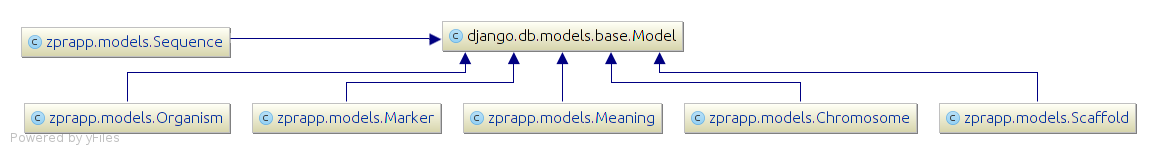
\includegraphics[width=1\textwidth]{grafika/model/final/model_diagram_klas2.png}
\caption{Diagram klas modelu danych.}
\label{diagram_klas_modelu}
\end{figure}

Każdy organizm posiada zbiór chromosomów, które mogą się składać z~wielu skafoldów. Skafoldy mają określoną kolejność w~chromosmie, znamy dodatkowo ich położenie i~długość. Ciąg zasad składający się na sekwencje jest ciałem skafoldu. Markery mogą być nanoszone na wybrany odcinek chromosomu z~przypisanym znaczeniem. Istotę obrazuje diagram zależności modelu (rys.\ref{diagram_zaleznosci_modelu}). Utworzona struktura relacyjna zaprezentowana została na rys.\ref{diagram_fizycznej_struktury}.
\begin{figure}[h]
\centering
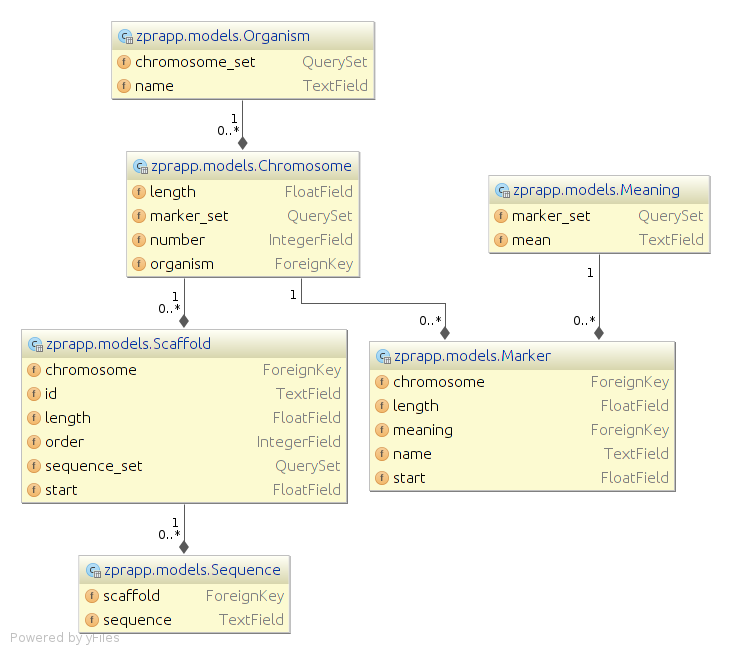
\includegraphics[width=0.9\textwidth]{grafika/model/final/model_diagram_zaleznosci_rozszerzony.png}
\caption{Diagram zależności modelu danych.}
\label{diagram_zaleznosci_modelu}
\end{figure}

\begin{figure}[h]
\centering
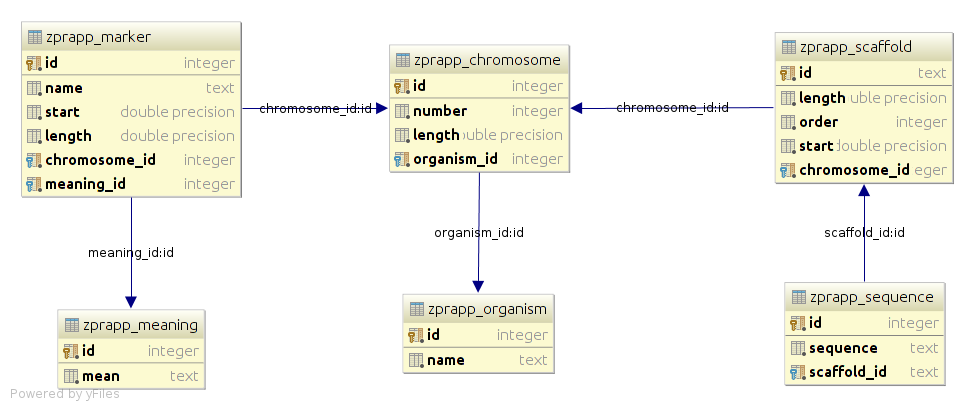
\includegraphics[width=1\textwidth]{grafika/diagram_bazy.png}
\caption{Diagram fizycznej struktury danych.}
\label{diagram_fizycznej_struktury}
\end{figure}

\subsubsection{Genom ogórka}
Baza danych została zainicjowana danymi o~genomie ogórka z~projektu \emph{WebOmicsViewer} autorstwa \emph{Piotra Róża}. Do realizacji zadania został mi  udostępniony backup bazy danych ww. pracy. Napotkałem problemy w~trakcie migracji danych, ponieważ okazały się one niespójne. Aby rozwiązać problem, zmuszony byłem dokonać analizy angażującej plik płaski xls, zawierający dodatkowe informacje o~skorelowanych markerach z~chromosomami. Moduł przeglądarki odpowiadający za inicjację bazy znajduje się w~pakiecie \emph{zpr.database}. Diagram klas został przedstawiony na rys.\ref{diagram_klas_budowy_bazy}. Klasa \emph{DatabaseGenome} agreguje obiekty pozostałych klas odpowiedzialnych za prawidłowe wyselekcjonowanie i~wstawienie danych do docelowej bazy.
\begin{figure}[h]
\centering
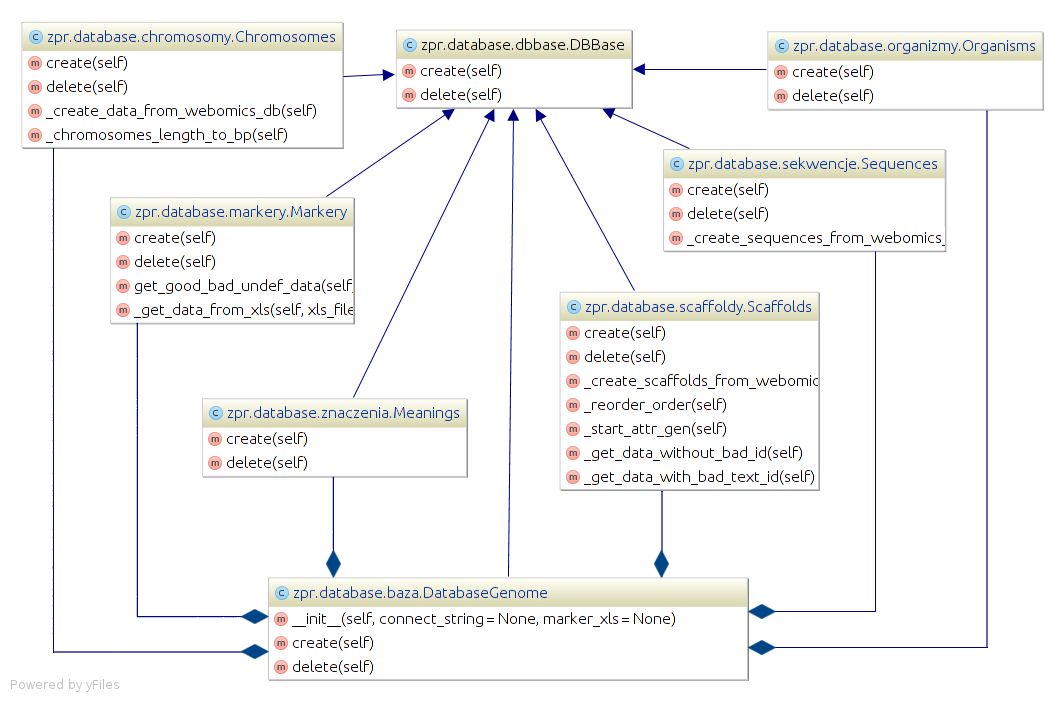
\includegraphics[width=1\textwidth]{grafika/model/final/budowa_bazy.png}
\caption{Diagram klas modułu odpowiedzialnego za inicjację bazy danymi ogórka.}
\label{diagram_klas_budowy_bazy}
\end{figure}

W~bazie przechowywanych jest 7 chromosomów ogórka, składających się łącznie z~964 skafoldów. Średnia długość przechowywanych skafoldów wynosi blisko 222 tysiące, zaś suma wszystkich sekwencji ponad 204 miliony par zasad. System bazodanowy gromadzi 72MB danych.


\subsection{Budowanie i~wdrażanie aplikacji}
Wdrażanie aplikacji na nową maszynę jest procesem żmudnym i~podatnym na błędy. Ręczne konfigurowanie środowiska zajmuje zazwyczaj wiele czasu. Niektóre czynności dają się z~powodzeniem zautomatyzować. Użyteczne klasy do tego celu znajdują się w~module \emph{\mbox{build\_tools}}. Klasa \emph{AppBuilder} zajmuje się m.in.:
\begin{itemize}
\item utworzeniem drzewa katalogów projektu
\item pobraniem plików potrzebnych do inicjacji bazy danych
\item ustawieniem parametru \emph{debug} (istotne przy wdrażaniu na środowisko produkcyjne)
\item utworzeniem środowiska \emph{virtualenv}, dzięki któremu mamy możliwość posiadania na tej samej maszynie kilku wersji tej samej biblioteki.
\end{itemize}
Klasa \emph{Deployer} zajmuje się głównie przygotowaniem aplikacji i~narzędzi do wdrożenia produkcyjnego. Generuje plik konfiguracyjny dla serwera WWW \emph{Nginx} oraz 
ze względów bezpieczeństwa tworzy nowy tajny klucz zabezpieczeń \emph{Django}. Obie klasy zostały przedstawione na rys.\ref{diagram_klas_appbuilder_deployer}.
Aplikacja została wdrożona na serwerze uczelnianym. Dostępna jest pod adresem:
\begin{center}
\url{http://smyrna.ise.pw.edu.pl:9002/}
\end{center} 
\begin{figure}[]
\centering
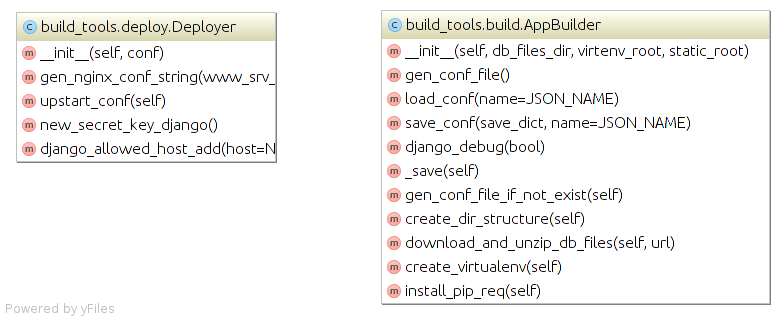
\includegraphics[width=1\textwidth]{grafika/model/final/appbuilder_deployer.png}
\caption{Diagram klas modułu \emph{build\_tools}.}
\label{diagram_klas_appbuilder_deployer}
\end{figure}

\subsection{Import i~export danych}
Jednym z~wymagań funkcjonalnych była możliwość przesyłania na serwer danych dotyczących nowych organizmów. Dane sekwencji powinny być zgodne z~formatem \emph{FASTA}\footnote{https://en.wikipedia.org/wiki/FASTA\_format}. Plik fasta powinien zawierać linię opisu zaczynającą się od znaku \verb|>|, a~w~niej identyfikator sekwencji. W~kolejnych wierszach ma znajdować się sekwencja (ATCG), aż do pojawienia się kolejnej linii ze znakiem \verb|>|, bądź osiągnięcia końca pliku.

Pozostałe pliki powinny być przesłane na serwer w~formacie \emph{GFF}\footnote{https://genome.ucsc.edu/FAQ/FAQformat.html\#format3}. Każdy rekord pliku GFF powinien rozpoczynać się \emph{id obiektu}, a~kończyć ewentualnym \emph{id} obiektu nadrzędnego, którego dotyczy. W~środku wymagane są kolejne atrybuty klasy.

Realizacja omawianego zadania wymaga po odebraniu plików, przeprowadzenia odpowiedniego procesu parsowania dokumentów po stronie serwera. Klasa potrafiąca generować pliki fasta i~gff, oraz je odbierać i~wkładać do bazy, znajduje się w~module \emph{zprapp.import\_export}, którego diagram klas został zaprezentowany na rys.\ref{diagram_klas_imp_exp}. Jeśli okaże się, że pliki nie spełniają wymaganych zależności, zostanie wygenerowany wyjątek informujący klienta na jakim etapie przetwarzania wydarzył się błąd.
\begin{figure}[h]
\centering
\includegraphics[width=1\textwidth]{grafika/model/final/imp_exp_diag_klass.png}
\caption{Diagram klas modułu \emph{import\_export}.}
\label{diagram_klas_imp_exp}
\end{figure}

\subsection{Trasowanie}
Aby korzystanie z~aplikacji było wygodne, warstwa prezentacji została stworzona w~idei stron typu \emph{one-page}. Podejście to cechuje wysoki poziom estetyki oraz duża interaktywność interfejsu. Niestety najczęściej przy takim rozwiązaniu pozbawiamy użytkownika możliwości zapisywania zakładek, ponieważ wszystkie operacje wykonują się dynamicznie bez zmiany adresu URL. Na szczęście \emph{AngularJS} jest narzędziem umożliwiającym uporanie się z~tym problemem. Listing \ref{routeprovider} przedstawia funkcję konfigurującą trasowanie URL w~przeglądarce. Do każdego widoku został przyporządkowany osobny kontroler ułatwiając pracę nad kodem.

\begin{figure}[h]
\centering
\renewcommand{\figurename}{Listing.}
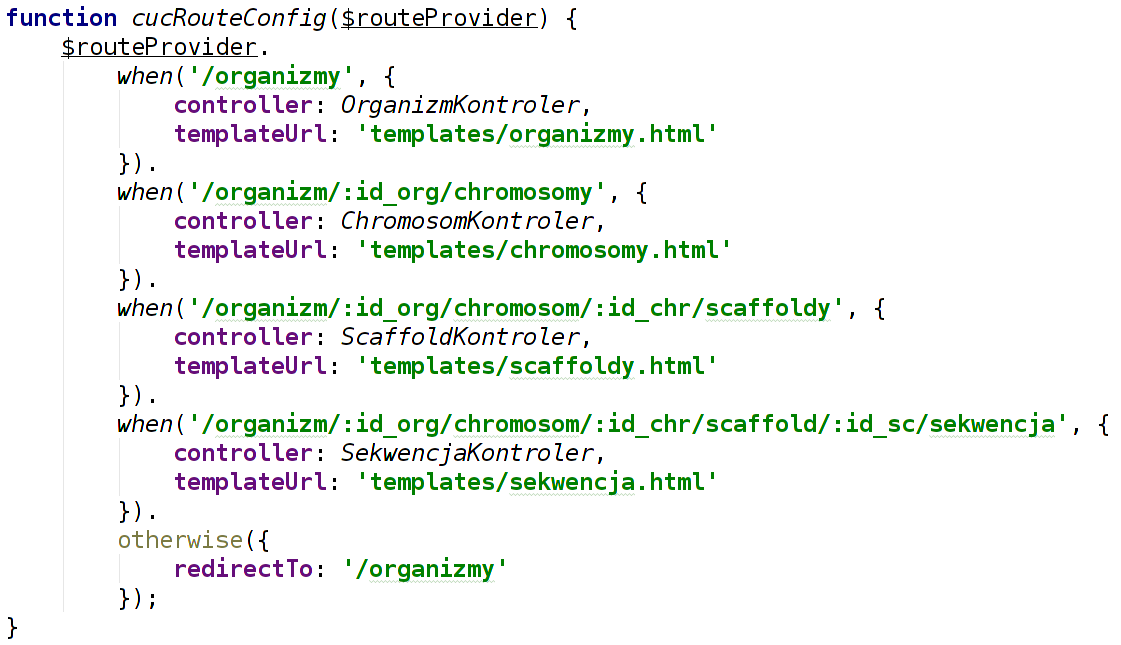
\includegraphics[width=1\textwidth]{grafika/routeProvider.png}
\caption{Funkcja konfigurująca trasowanie URL w~przeglądarce WWW.}
\label{routeprovider}
\end{figure}

\section{Testowanie}
Etap testowania oprogramowania to czas, w~którym badamy całość programu lub jego poszczególne komponenty, uruchamiając kod w~kontrolowanych warunkach i~sprawdzając rezultaty. Przeprowadzając testy sprawdzamy czy wyniki są zgodne z~oczekiwaniami użytkownika, gwarantując tym samym wymaganą jakość oprogramowania. Niejednokrotnie podczas implementacji, zastosowanie testów pomogło mi na wczesnym etapie wykryć defekty aplikacji, nie propagując błędów. Testy przeprowadzałem na dwóch poziomach: 
\begin{itemize}
\item testowania jednostkowego
\item testowania funkcjonalnego.
\end{itemize}

\subsection{Testy jednostkowe}
Przedmiotem testowania jednostkowego (ang. \emph{unit testing}) są podstawowe jednostki programu. Postacie sprawdzanych komponentów różnią się w~zależności od implementacji. Weryfikować możemy poprawność pojedynczych funkcji, metod czy klas zapisanych w~języku obiektowym. Celem testowania na tym poziomie jest potwierdzenie poprawności wykonywanych fragmentów aplikacji jednocześnie próbując znaleźć jak największą liczbę błędów. Przeprowadziłem łącznie 26 testów jednostkowych.

\subsubsection{Przykład testu widoku}
Funkcja widoku \emph{ajaxSeqSection(request)} będąca po stronie serwera ma za zadanie zwrócić fragment sekwencji chromosomu, który użytkownik zażąda korzystając z~graficznego interfejsu użytkownika. Odnajdując potrzebne skafoldy musi je przyciąć w~odpowiedni sposób, połączyć w~całość w~zadanym zakresie wypełniając luki między nimi i~odesłać do klienta.

Aby proces przeprowadzać w~stałych kontrolowanych warunkach, przed każdym uruchomieniem zestawu testów dla omawianego widoku tworzona jest testowa baza danych o~strukturze identycznej jak w~środowisku produkcyjnym lecz z~innymi, niezmieniającymi się danymi. Funkcja realizująca wspomnianą czynność przedstawiona na listingu \ref{unit_test_db}

\begin{figure}[!h]
\centering
\renewcommand{\figurename}{Listing.}
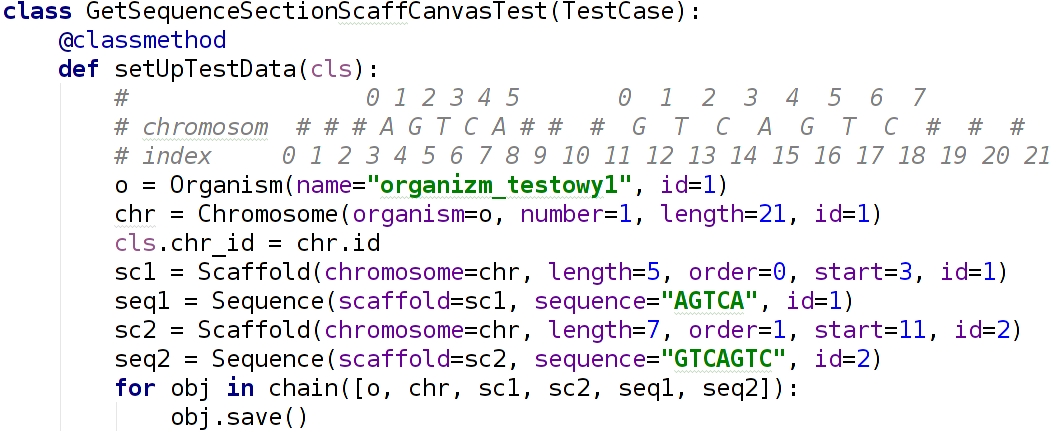
\includegraphics[width=0.83\textwidth]{grafika/testowa_bd_unit_test.png}
\caption{Funkcja tworząca testową bazę danych dla zestawu testów \emph{GetSequenceSectionScaffCanvasTest}}
\label{unit_test_db}
\end{figure}

Przeprowadzanie eksperymentów dla wszystkich możliwych danych wejściowych byłoby bardzo niewygodne. Projektując testy dla omawianego przykładu starałem się tak dobrać zbiór przypadków testowych aby efektywnie sprawdzić wszystkie aspekty poprawności funkcji widoku. Wyniki 13 przypadków testowych przedstawione na rys.\ref{testy_jednostkowe_pycharm}.

\begin{figure}[!h]
\centering
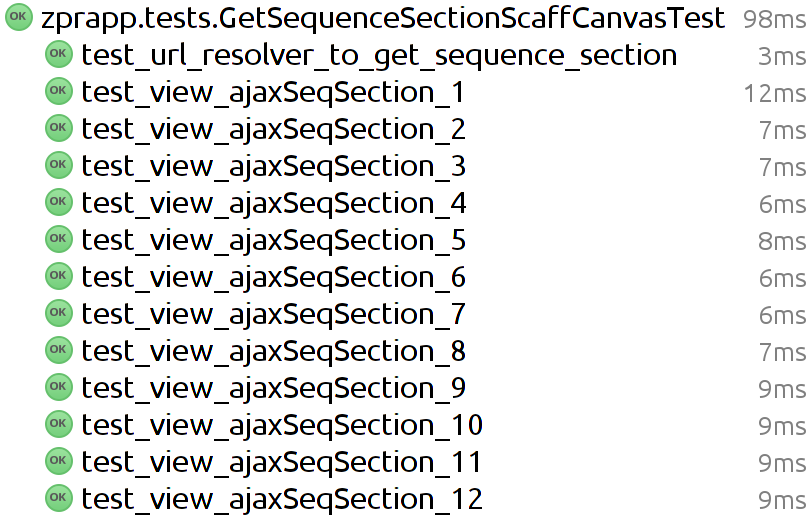
\includegraphics[width=0.6\textwidth]{grafika/testy_jednostkowe_wyniki_pycharm.png}
\caption{Wynik testów jednostkowych widoku \emph{ajaxSeqSection} prezentowany w~IDE.}
\label{testy_jednostkowe_pycharm}
\end{figure}

\subsection{Testy funkcjonalne}
Tego rodzaju testy sprawdzają z~zewnątrz sposób działania całej aplikacji. Nazywane są często \emph{testami czarnej skrzynki}, ponieważ osoba testująca nie korzysta z~wiedzy dotyczącej wewnętrznych komponentów sprawdzanego systemu, lecz opiera się na założeniach funkcjonalnych jakie aplikacja powinna spełniać zgodnie z~założeniami wynikającymi z~wymagań.

Do przeprowadzenia testów funkcjonalnych skorzystałem z~narzędzia \emph{Selenium}, które pozwala na zaprzęgnięcie do nich prawdziwej przeglądarki WWW. Łącznie wykonałem 12 testów funkcjonalnych. Przebieg przykładowego testu symuluje potencjalne działania użytkownika w~trakcie korzystania z~aplikacji.

\subsubsection{Przykład}
Scenariusz przeprowadzonego testu przedstawionego na listingu \ref{test_funkcjonalny}:
\begin{enumerate}
\item Użytkownik wchodzi na stronę główną aplikacji.
\item Zauważa ładnie wyświetlony pasek z~tytułem aplikacji.
\item Wybiera pierwszy organizm.
\item Decyduje się na wybór drugiego chromosomu.
\item Ustawia parametry widoku aby pokazywały część chromosomu od indeksu 10 do 20.
\item Wybiera pożądany skafold.
\item Klika w~przycisk służący do kopiowania w~celu zapisania sekwencji skafoldu do schowka systemowego.
\item Wyłącza aplikację.
\end{enumerate}

Rezultaty testu są pozytywne, wykonanie zajęło ponad 7 sekund (rys.\ref{wynik_testu_funkcjonalnego}).

\begin{figure}[!h]
\centering
\renewcommand{\figurename}{Listing.}
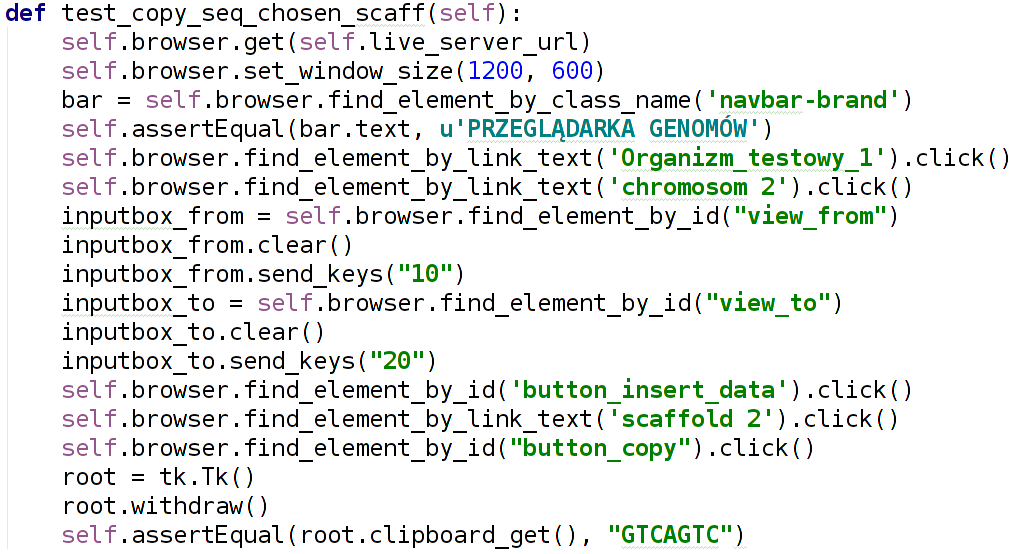
\includegraphics[width=0.8\textwidth]{grafika/test_funkcjonalny.png}
\caption{Przykładowy test funkcjonalny aplikacji.}
\label{test_funkcjonalny}
\end{figure}

\begin{figure}[!h]
\centering

\includegraphics[width=0.4\textwidth]{grafika/test_funk_wynik_pycharm.png}
\caption{Wynik przykładowego testu funkcjonalnego w~środowisku PyCharm.}
\label{wynik_testu_funkcjonalnego}
\end{figure}

\chapter{Demonstracja programu}
Na stronie startowej aplikacji, wyświetlane są dostępne organizmy w~bazie danych oraz przycisk umożliwiający uruchomienie okna dialogowego pozwalającego na dodanie nowego organizmu (rys.\ref{home}). Wybierając organizm, przechodzimy do widoku chromosomów (rys.\ref{chromosomy}). Przejście do następnego widoku (rys.\ref{skafoldy}) następuje po kliknięciu w~wybrany słupek reprezentujący chromosom. W~tej części aplikacji nawigujemy po chromosomie za pomocą  przycisków przybliżania i~poruszania się na boki w~celu odnalezienia pożądanego fragmentu genomu. Potrafimy nanosić na główny pasek poszczególne markery. Aby odczytać fragment wyświetlanej sekwencji należy nacisnąć przycisk z~okiem, bądź wybrać z~tabeli skafold, którego zawartość będziemy chcieć pobrać.
\vspace{3cm}
\begin{figure}[!h]
\centering
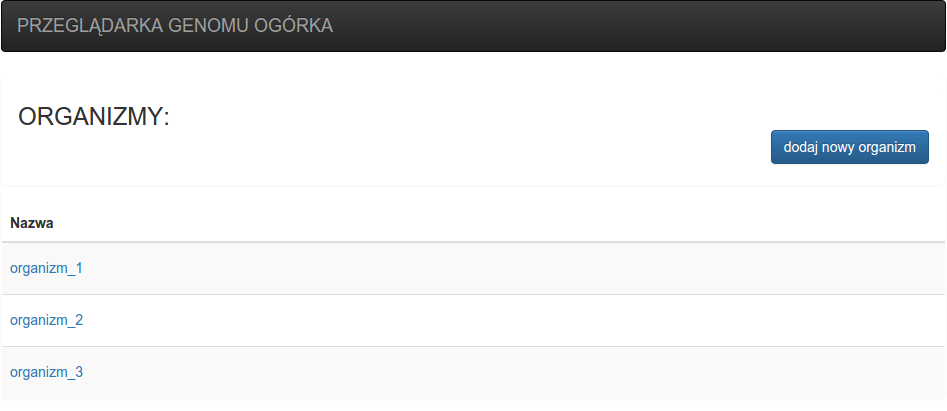
\includegraphics[width=1\textwidth]{grafika/home.png}
\caption{Widok strony startowej.}
\label{home}
\end{figure}
\begin{figure}[!h]
\centering
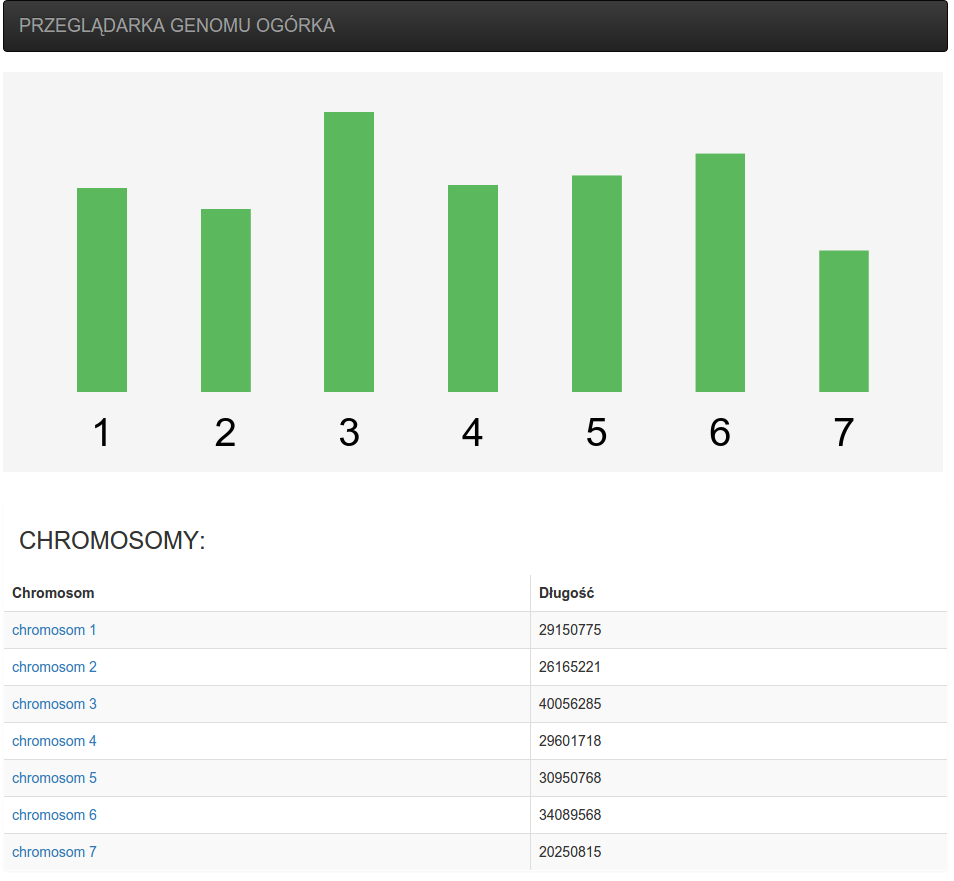
\includegraphics[width=1\textwidth]{grafika/chromosomy.png}
\caption{Widok chromosomów organizmu.}
\label{chromosomy}
\end{figure}
\begin{figure}[!h]
\centering
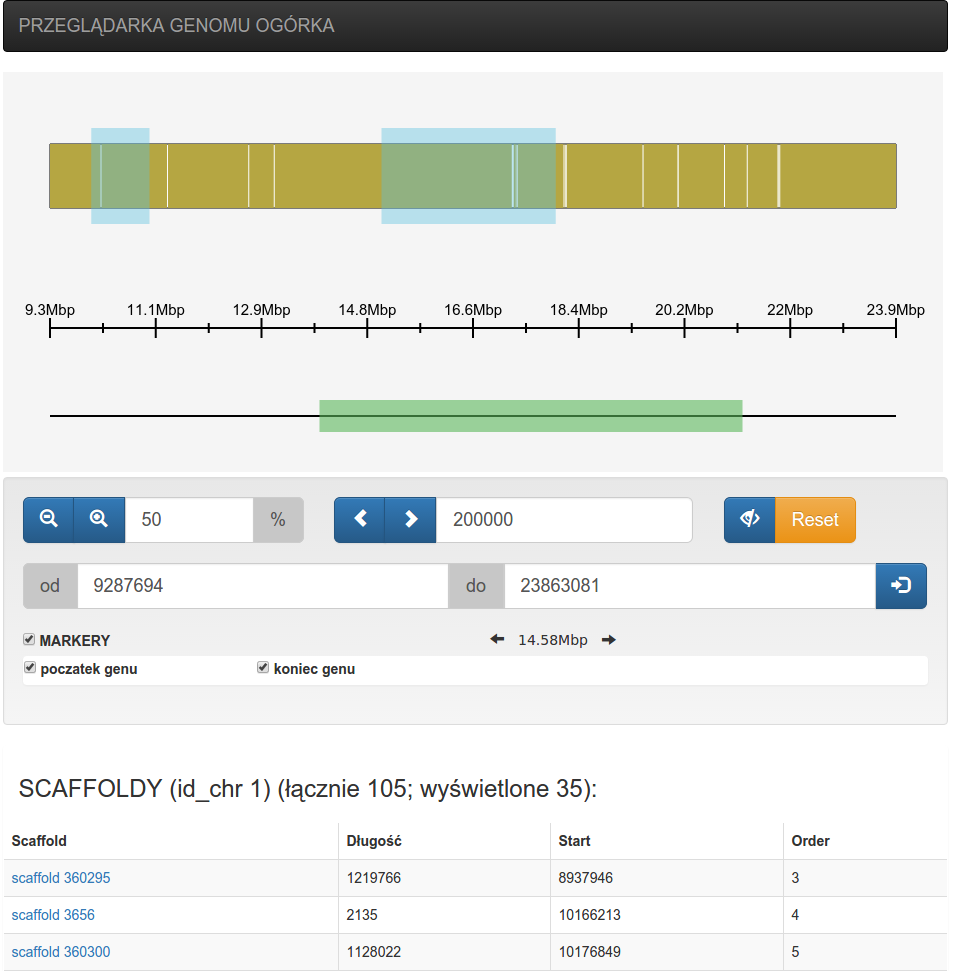
\includegraphics[width=1\textwidth]{grafika/skafoldy.png}
\caption{Widok skafoldów chromosomu.}
\label{skafoldy}
\end{figure}


\chapter{Podsumowanie}
Wartość przedmiotowej pracy inżynierskiej w~opinii autora można przedstawić w~dwóch zasadniczych wymiarach.

Po pierwsze, zaproponowana przeglądarka genomów, możne być wykorzystywana jako użyteczny element pomocniczy w~procesach badawczych, które w~istotny sposób przyczyniają się do postępu cywilizacyjnego. Osiągnięcia genomiki dają np. możliwość pożądanych modyfikacji roślin, usprawniają kryminalistykę i~sądownictwo (analiza śladów biologicznych, identyfikacja zmarłych, ustalanie ojcostwa), pozwalają na określanie stopnia pokrewieństwa pomiędzy gatunkami oraz wpływają na rozwój precyzyjnej diagnostyki medycznej opartej na metodach genetyki molekularnej.

Inna, osobista wartość wynika z~faktu poszerzenia umiejętności autora w~zakresie tworzenia aplikacji sieciowych. W~trakcie pisania pracy napotkałem wiele problemów, których rozwiązywanie nauczyło mnie pokory i~pozwoliło poznać wiele ciekawych technologii. Zapoznanie się z~całym wachlarzem nowoczesnych narzędzi było istotnym etapem na drodze do zawodu programisty i~stanowiło ważne uzupełnienie wiedzy zdobytej podczas studiów na Wydziale Elektroniki i~Technik Informacyjnych. Nabyte umiejętności będę wykorzystywał w~przyszłych projektach, doskonaląc się w~sztuce inżynieryjnej. 

Otwartą możliwością i~kwestią ewentualnej przyszłości pozostaje rozwinięcie funkcjonalności zaproponowanej przeglądarki o~możliwość przeprowadzania analiz statystycznych i~porównawczych z~wykorzystaniem publicznie dostępnych baz danych. Architektura przeglądarki została tak zaprojektowana by możliwe było w~przyszłości implementowanie wysokowydajnych algorytmów z~użyciem języków kompilowanych takich jak \emph{C++}. Dzięki bibliotece \href{http://www.boost.org/}{\emph{Boost}}, część serwerowa napisana w~Pythonie z~powodzeniem może być łączona z~kodem \emph{C++}, oferując ogromne możliwości rozbudowy aplikacji, która w~mojej opinii posiada potencjał aby w~przyszłości, po rozszerzeniu funkcjonalności, konkurować z~innymi projektami.

Jednym z~najpopularniejszych warzyw w~Polsce i~na świecie jest ogórek. Duży popyt powoduje, że ogórek był i~nadal pozostaje ważnym obiektem upraw a~więc i~badań. Ogórek należy do rodziny dyniowatych, jest spokrewniony z~melonem, arbuzem i~dynią. W~celu zsekwencjonowania jego genomu, w 2008r. zostało powołane Polskie Konsorcjum Sekwencjonowania Genomu Jądrowego Ogórka (rys.\ref{konsorcjum}). Konsorcjum jest wspólnym przedsięwzięciem naukowców i~przedsiębiorców z~różnych instytucji chętnych do współpracy w~procesie eksploracji genomu ogórka. Głównym zadaniem wskazanego konsorcjum jest postęp nad składaniem i wykorzystaniem sekwencji genomu do badań i~aplikacji. Istnieje szansa, że przeglądarka stworzona w ramach pracy dyplomowej będzie w przyszłości intensywnie używana przez ww. związek przedsiębiorstw. Możliwe, że aplikacja po rozszerzeniu funkcjonalności i optymalizacji interfejsu użytkownika, jako narzędzie, przyczyni się do utrzymania hodowli ogórka w Polsce na poziomie konkurencyjnym do światowego.\cite{konsorcjium-pdf, pcc-genomics}

\begin{figure}[h]
\centering

\includegraphics[width=0.3\textwidth]{grafika/loga/konsorcjum.png}
\caption{Logo Polskiego Konsorcjum Sekwencjonowania Genomu Jądrowego Ogórka (ang. \emph{Polish Consortium of Cucumber Genome Sequencing}).}
\label{konsorcjum}
\end{figure}


%%%%%%%%%%%%%%%%%%%%%%%%%%%%%%%%%%%%%%%%%%%%%%%%%%%%%%%%%%%%%  
% BIBLIOGRAFIA
%%%%%%%%%%%%%%%%%%%%%%%%%%%%%%%%%%%%%%%%%%%%%%%%%%%%%%%%%%%%%
\begin{thebibliography}{99}
%\bibitem{pl-wiki-bioinf} Wikipedia (PL) \emph{Bioinformatyka}\\ \url{https://pl.wikipedia.org/wiki/Bioinformatyka}, \mbox{15~sierpnia~2015}
%\bibitem{e-biotech-wycisnac_sekw} e-Biotechnologia \emph{Co można wycisnąć ze zwykłej sekwencji?}\\
%\url{http://www.e-biotechnologia.pl/Artykuly/Co-mozna-wycisnac-ze-zwyklej-sekwencji/} \mbox{1~stycznia~2016}
%\bibitem{biotech-uwm} %dr
%Jan Paweł Jastrzębski \emph{Wykład 2 bioinformatyka 2007/2008}\\
%\url{http://ebiolog.pl/graf/Wyklady/biotech/W2/Bioinformatyka_W2.pdf}, \mbox{16~sierpnia~2015}
%\bibitem{pl-wiki-cM} Wikipedia (PL) \emph{Centymorgan}\\ \url{https://pl.wikipedia.org/wiki/Centymorgan}, \mbox{15~sierpnia~2015}
%\bibitem{e-biotech-map-gen} e-Biotechnologia \emph{Mapowanie genomów}\\ \url{http://www.e-biotechnologia.pl/Artykuly/Mapowanie-genomow}, \mbox{15~sierpnia~2015}
%\bibitem{e-biotech-encykl-pz} e-Biotechnologia, Encyklopedia \emph{Para zasad}\\ \url{http://www.e-biotechnologia.pl/encyklopedia/articles.php?lng=pl&pg=175}, \mbox{15~sierpnia~2015}
%\bibitem{en-wiki-gen_bro} Wikipedia (EN) \emph{Genome browser}\\ \url{https://en.wikipedia.org/wiki/Genome_browser}, \mbox{16~sierpnia~2015}
%\bibitem{historia-bioinf} Uniwersytet Warmińsko Mazurski w~Olsztynie \emph{Historia Bioinformatyki...}\\ \url{http://www.uwm.edu.pl/wnz/KBZ/Lipazy/bioinfo-historia.html}
%\bibitem{pl-wiki-kwas-rybonukleinowy} Wikipedia (PL) \emph{Kwas rybonukleinowy}\\
%\url{https://pl.wikipedia.org/wiki/Kwasy_rybonukleinowe} \mbox{16~sierpnia~2015}
%\bibitem{pl-wiki-soap} Wikipedia (PL) \emph{SOAP}\\
%\url{https://pl.wikipedia.org/wiki/SOAP}, \mbox{17~sierpnia~2015}
%\bibitem{pl-wiki-rest} Wikipedia (PL) \emph{REST}\\
%\url{https://pl.wikipedia.org/wiki/Representational_State_Transfer}, \mbox{17~sierpnia~2015}
%\bibitem{pdf-politech-poz} Anna Leśniewska \emph{Przeglądarki genomowe (2)}\\
%\url{http://www.cs.put.poznan.pl/alesniewska/BABD/W_2015-05-06.pdf}, \mbox{17~sierpnia~2015}
%\bibitem{pl-wiki-apache} Wikipedia (PL) \emph{Apache License}\\ \url{https://pl.wikipedia.org/wiki/Apache_License}, \mbox{17~sierpnia~2015}		
%\bibitem{pdf-mimuw} Bartek Wilczyński \emph{Architektura dużych projektów bioinformatycznych}\\
%\url{http://bioputer.mimuw.edu.pl/~bartek/APB/wyk3-browsers.pdf}, \mbox{17~sierpnia~2015}
%\bibitem{bioweb} Robert M. Nowak \emph{Polyglot programming the applications to analyze genetic data} BioMed Research International, vol. 2014, doi:10.1155/2014/253013, \url{http://www.hindawi.com/journals/bmri/2014/253013} \mbox{10~październik~2015}
%\bibitem{pl-wiki-biopolimer} Wikipedia (PL) \emph{Biopolimery}\\ \url{https://pl.wikipedia.org/wiki/Biopolimery}, \mbox{11~październik~2015}
%\bibitem{pl-wiki-nukl} Wikipedia (PL) \emph{Nukleotydy}\\ \url{https://pl.wikipedia.org/wiki/Nukleotydy}, \mbox{11~październik~2015}
%\bibitem{pl-wiki-bialka} Wikipedia (PL) \emph{Białka}\\ \url{https://pl.wikipedia.org/wiki/Bia%C5%82ka}, \mbox{11~październik~2015}
%\bibitem{pl-wiki-2nd-struct} Wikipedia (PL) \emph{Struktura drugorzędowa białka}\\ \url{https://pl.wikipedia.org/wiki/Struktura_drugorz%C4%99dowa_bia%C5%82ka}, \mbox{11~październik~2015}
%\bibitem{e-biotech-bialka} e-Biotechnologia \emph{Budowa białek}\\ \url{http://www.e-biotechnologia.pl/Artykuly/budowa-bialek}, \mbox{11~październik~2015}
%\bibitem{inz-opr-k.sacha} Krzysztof Sacha \emph{Inżynieria oprogramowania} PWN, Warszawa 2010
%\bibitem{IEEE-wymagania}IEEE/ANSI Std 610, Glossary of Software Engineering Terminology, IEEE Computer Society Press 1990. %str62 o~wymaganiach
%\bibitem{learning-python} Mark Lutz \emph{Learning Python, 5th Edition}\\
%O'Reilly Media, June 2013. ISBN: 978-1-449-35573-9.
%\bibitem{django-girls} \emph{Django Girls}\\
%\url{http://tutorial.djangogirls.org/pl/django/index.html} \mbox{15~stycznia~2015}
%\bibitem{django} \emph{Django}\\
%\url{https://www.djangoproject.com/} \mbox{15~stycznia~2015}
%\bibitem{gunicorn} \emph{Gunicorn}\\
%\url{http://gunicorn.org/} \mbox{14~stycznia~2015}
%\bibitem{en-wiki-wsgi} Wikipedia (EN) \emph{WSGI}\\
%\url{https://en.wikipedia.org/wiki/Web_Server_Gateway_Interface} \mbox{14~stycznia~2015}
%\bibitem{nginx} Nginx\\
%\url{https://www.nginx.com/resources/wiki/} \mbox{14~stycznia~2015}
%\bibitem{pycharm} JetBrains \emph{PyCharm}\\
% wikipedia PL PyCharm, Django, Python
%\url{https://www.jetbrains.com/pycharm/}, \mbox{14~stycznia~2015}
%\bibitem{python_i_django} Jeff Forcier, Paul Bissex, Wesley Chun \emph{Python i Django. Programowanie aplikacji webowych.}\\
%Helion, 2009. ISBN 978-83-246-2225-2.
%\bibitem{git}Włodzimierz Gajda \emph{Git. Rozproszony system kontroli wersji}\\
%Helion, 2013. ISBN 978-83-246-7305-6.
%\bibitem{it-pwn-aplikacje-trojwartwowe} PWN \emph{Po co dzielić aplikacje na warstwy?}\\ \url{http://it.pwn.pl/Artykuly/Programowanie/Po-co-dzielic-aplikacje-na-warstwy} \mbox{20~stycznia~2016}

%!!!!!!!!!!!!!!!!!!!!!!!!!!!!!!!!!!!!!!!!!!!!!!!!!!!!!!!!!!!!!!! 
% NOWA BIBLIOGRAFIA !!!!!!!!!!!!!!!!!!!!!!!!!!!!!!!!!!!!!!!!!!!!
%!!!!!!!!!!!!!!!!!!!!!!!!!!!!!!!!!!!!!!!!!!!!!!!!!!!!!!!!!!!!!!!
\bibitem{nature}Sanger F, Air GM, Barrell BG, Brown NL, Coulson AR, Fiddes CA, Hutchison CA, Slocombe PM, Smith M., \emph{Nucleotide sequence of bacteriophage phi} X174 DNA, Nature. 1977 Feb 24;265(5596):687-95.
\bibitem{bioweb} Robert M. Nowak \emph{Polyglot programming the applications to analyze genetic data} BioMed Research International, vol. 2014, doi:10.1155/2014/253013, \url{http://www.hindawi.com/journals/bmri/2014/253013} \mbox{10~październik~2015}
\bibitem{pdf-mimuw} Bartek Wilczyński \emph{Architektura dużych projektów bioinformatycznych}\\
\url{http://bioputer.mimuw.edu.pl/~bartek/APB/wyk3-browsers.pdf}, \mbox{17~sierpnia~2015}
\bibitem{inz-opr-k.sacha} Krzysztof Sacha \emph{Inżynieria oprogramowania} PWN, Warszawa 2010
\bibitem{biotech-uwm} %dr
Jan Paweł Jastrzębski \emph{Wykład 2 bioinformatyka 2007/2008}\\
\url{http://ebiolog.pl/graf/Wyklady/biotech/W2/Bioinformatyka_W2.pdf}, \mbox{16~sierpnia~2015}
\bibitem{pdf-politech-poz} Anna Leśniewska \emph{Przeglądarki genomowe (2)}\\
\url{http://www.cs.put.poznan.pl/alesniewska/BABD/W_2015-05-06.pdf}, \mbox{17~sierpnia~2015}
\bibitem{historia-bioinf} Uniwersytet Warmińsko Mazurski w~Olsztynie \emph{Historia Bioinformatyki...}\\ \url{http://www.uwm.edu.pl/wnz/KBZ/Lipazy/bioinfo-historia.html}
\bibitem{IEEE-wymagania}IEEE/ANSI Std 610, Glossary of Software Engineering Terminology, IEEE Computer Society Press 1990. %str62 o~wymaganiach
\bibitem{learning-python} Mark Lutz \emph{Learning Python, 5th Edition}\\
O'Reilly Media, June 2013. ISBN: 978-1-449-35573-9.
\bibitem{django-girls} \emph{Django Girls}\\
\url{http://tutorial.djangogirls.org/pl/django/index.html} \mbox{15~stycznia~2015}
\bibitem{django} \emph{Django}\\
\url{https://www.djangoproject.com/} \mbox{15~stycznia~2015}
\bibitem{gunicorn} \emph{Gunicorn}\\
\url{http://gunicorn.org/} \mbox{14~stycznia~2015}
\bibitem{nginx} Nginx\\
\url{https://www.nginx.com/resources/wiki/} \mbox{14~stycznia~2015}
\bibitem{pycharm} JetBrains \emph{PyCharm}\\
% wikipedia PL PyCharm, Django, Python
\url{https://www.jetbrains.com/pycharm/}, \mbox{14~stycznia~2015}
\bibitem{python_i_django} Jeff Forcier, Paul Bissex, Wesley Chun \emph{Python i~Django. Programowanie aplikacji webowych.}\\
Helion, 2009. ISBN 978-83-246-2225-2.
\bibitem{git}Włodzimierz Gajda \emph{Git. Rozproszony system kontroli wersji}\\
Helion, 2013. ISBN 978-83-246-7305-6.
\bibitem{e-biotechnologia} e-Biotechnologia \emph{Co można wycisnąć ze zwykłej sekwencji?, Mapowanie genomów, Para zasad, Budowa białek}\\ \url{http://www.e-biotechnologia.pl/}
\bibitem{wikipedia-pl} Wikipedia(PL) \emph{Bioinformatyka, Centymorgan, Kwas rybonukleinowy, SOAP, REST, Apache License, Biopolimery, Nukleotydy, Białka, Struktura drugorzędowa białka, PyCharm, Django, Python, Chromosom, JavaScript, HTML5, Testowanie oprogramowania, Genom} \\ \url{http://pl.wikipedia.org/}
\bibitem{wikipedia-en} Wikipedia(EN) \emph{Genome browser, WSGI, Contig} \\ \url{http://en.wikipedia.org/}
\bibitem{pwn-encyklopedia} PWN \emph{Chromosomy, Marker genetyczny} \\ \url{http://encyklopedia.pwn.pl/haslo/chromosomy;3886021.html}
\bibitem{medicinenet} Medicinenet \emph{Definition of Scaffold} \\ \url{http://www.medicinenet.com/script/main/art.asp?articlekey=25223} \mbox{21~stycznia~2015}
\bibitem{it-pwn} IT PWN \emph{Po co dzielić aplikacje na warstwy?,\\ Dlaczego warto stosować różne języki programowania jednocześnie?}\\ \url{http://it.pwn.pl/Artykuly/Programowanie/} \mbox{20~stycznia~2016}
\bibitem{javascript}Jon Duckerr \emph{JavaScript and JQuery: Interactive Front-End Web Development}\\ John Wiley \& Sons, Inc., Indianapolis, Indiana, 2014. ISBN 978-83-283-0126-9.
\bibitem{angular}Adam Freeman \emph{AngularJS Profesjonalne techniki}\\ Helion, 2014. ISBN 978-83-283-0200-6.
\bibitem{bootstrap}Syed Fazle Rahman \emph{Bootstrap. Tworzenie interfejsów stron WWW. Technologia na start!}\\ Helion, 2015. ISBN 978-83-283-0514-4.
\bibitem{tdd}Harry J.W. Percival \emph{TDD w~praktyce. Niezawodny kod w~języku Python}
%\bibitem{PAN_RUN}Polska Akademia Nauk, Rada Upowszechniania Nauki, \emph{Sukces polskich genetyków} \\ \url{http://www.run.pan.pl/index.php/194-sukces-polskich-genetykow} \mbox{27~stycznia~2015}
\bibitem{konsorcjium-pdf} Zbigniew Przybecki, Rafał Wóycicki, Stefan Malepzszy \emph{Sekrety ogórka nareszcie ujawnione - genom ogórka zsekwencjonowany}, tom 36, 2009 suplement nr 25 (19-31)
\bibitem{pcc-genomics} PCC Genomics \\ \url{http://csgenome.sggw.pl/en-us/} \mbox{27~stycznia~2015}
\end{thebibliography}
\end{document}